\documentclass[12pt,a4paper]{article}

% =================================================
% Font (XeLaTeX or LuaLaTeX REQUIRED)
% =================================================
\usepackage{fontspec}
\setmainfont{Trebuchet MS}

\usepackage{listings}
\usepackage{xcolor}
\usepackage{subcaption}

\lstset{
    language=Python,
    basicstyle=\ttfamily\small,
    keywordstyle=\color{blue},
    stringstyle=\color{red},
    commentstyle=\color{gray},
    showstringspaces=false,
    breaklines=true,
    frame=single
}

% =================================================
% Math and symbols
% =================================================
\usepackage{amsmath,amssymb,amsfonts}

% =================================================
% Graphics and floats
% =================================================
\usepackage{graphicx}
\usepackage{float}
\usepackage{placeins}

\usepackage{hanging}
\usepackage{ragged2e}

% =================================================
% Tables
% =================================================
\usepackage{booktabs}
\usepackage{multirow}
\usepackage{array}

% =================================================
% Lists and layout
% =================================================
\usepackage{enumitem}
\usepackage{geometry}
\geometry{margin=1in}

% =================================================
% Algorithms                              ← NEW
% =================================================
\usepackage{algorithm}
\usepackage{algpseudocode}

% Rename float label to match document style
\floatname{algorithm}{Algorithm}

% Typographic helpers used in algorithm bodies
\newcommand{\kw}[1]{\textbf{#1}}
\newcommand{\ty}[1]{\texttt{#1}}
\newcommand{\cmt}[1]{\textcolor{gray}{$\triangleright$ \textit{#1}}}
\algrenewcommand{\algorithmiccomment}[1]{\hfill\cmt{#1}}

% =================================================
% TOC customization
% =================================================
\usepackage[titles]{tocloft}
\renewcommand{\cftsecleader}{\cftdotfill{\cftdotsep}}

% =================================================
% Citations
% =================================================
\usepackage{cite}

% =================================================
% Hyperlinks (no colors, no boxes)
% =================================================
\usepackage[hidelinks]{hyperref}


% =================================================
% pdf imports
% =================================================
\usepackage{pdfpages}

% =================================================
% Title (UNCHANGED AS REQUESTED)
% =================================================
\title{
\textbf{Final Dissertation Report}\\[0.5em]
Adaptive Multi-LLM Agentic RAG with Dynamic Task Routing and Retrieval Planning
}

\author{Partha Pratim Mazumder}
\date{}



\begin{document}

% ---------------- Custom Title Page ----------------
\begin{titlepage}
    \centering

    % University logo
    
\includegraphics[width=0.3\textwidth]{../assets/solent_logo.png}\\[0.8cm]

    {\LARGE \textbf{SOLENT UNIVERSITY SOUTHAMPTON}}\\[0.4cm]
    {\large School of Technologies and Maritime Industries}

    \vspace{1.5cm}

    {\Large \textbf{Dissertation - Research Project (COM726)}}\\[0.4cm]
    {\large \textbf{Final Dissertation Report}}\\[0.2cm]
    {\small \textbf{Academic Year 2025--2026}}

    \vspace{1.5cm}

    % ===== Preserved Title =====
    {\Huge \textbf{Adaptive Multi-LLM Agentic RAG}}\\[0.3cm]
    {\Large \textbf{with Dynamic Task Routing and Retrieval Planning}}

    \vspace{1.5cm}

    {\Large \textbf{Partha Pratim Mazumder}}\\[0.2cm]
    {\large Student ID: Q103063737}\\[0.1cm]
    {\small \texttt{0mazup37@solent.ac.uk}}

    \vspace{1.2cm}

    {\large \textbf{Module Leader: Dr Bacha Rehman}}\\[0.3cm]
    {\large \textbf{Submission Date: \today}}

    \vspace{0.8cm}

    {\footnotesize \copyright~Solent University, \the\year}

\end{titlepage}

% =================================================
% Front Matter
% =================================================
\pagenumbering{roman}


% ---- Table of Contents ----
\tableofcontents
\newpage

% ---- List of Figures ----
\listoffigures
\addcontentsline{toc}{section}{List of Figures}
\newpage

% ---- List of Tables ----
\listoftables
\addcontentsline{toc}{section}{List of Tables}
\newpage

% ---- List of Listings ----
\lstlistoflistings
\addcontentsline{toc}{section}{List of Listings}
\newpage

% ---- List of Algorithms ----          ← NEW
\listofalgorithms
\addcontentsline{toc}{section}{List of Algorithms}
\newpage



% ---- Abstract ----
\newpage
\section*{Abstract}
\addcontentsline{toc}{section}{Abstract}

The rapid growth of large language models (LLMs) creates both opportunities and challenges for scalable conversational AI. Most current systems rely on monolithic pipelines that apply uniform inference strategies, leading to inefficiencies, increased hallucination risk, and underutilisation of diverse model strengths. This dissertation presents an Adaptive Multi-LLM Agentic Retrieval-Augmented Generation (RAG) system that addresses these limitations through dynamic task routing, specialist model selection, and selective retrieval.

Built on LangGraph, the system integrates ten heterogeneous open-weight and API-based models. A central orchestration layer classifies queries by task type and complexity, routing them to one of three execution paths: direct inference, retrieval-augmented generation using a ChromaDB vector store, or agentic multi-step execution with web search and computational tools. State persistence is managed via a MySQL-backed checkpointing mechanism, enabling resumable multi-turn interactions.

The system is evaluated on the HotpotQA and MuSiQue multi-hop question-answering benchmarks using metrics including Exact Match, F1 Score, Retrieval Precision, Routing Accuracy, and response latency. A companion Android application extends functionality via a REST API. Key contributions include an intent-aware routing architecture, adaptive specialist model selection, and evidence that selective retrieval reduces hallucinations compared to always-on approaches. Results demonstrate that adaptive multi-LLM orchestration outperforms monolithic baselines in both accuracy and computational efficiency, supporting the core research thesis.

\newpage


% =================================================
% Main Content
% =================================================
\pagenumbering{arabic}

\section{Introduction}
\label{sec:introduction}

Recent advances in large language models (LLMs) have transformed artificial intelligence, enabling systems capable of sophisticated reasoning, code generation, and instruction following (Brown et al., 2020; Wei et al., 2022). Models such as GPT-4, LLaMA, Mistral, and Gemini have democratised access to generative capabilities and spurred interest in production-grade AI assistants across diverse domains (Touvron et al., 2023; Jiang et al., 2023; Team et al., 2024).

Despite these advances, most deployed systems rely on monolithic pipelines in which a single model handles all queries uniformly, regardless of task complexity or retrieval requirements (Singh et al., 2025). This is inherently suboptimal: simple queries incur unnecessary retrieval overhead, while complex multi-hop tasks may fail without structured external knowledge. Retrieval-Augmented Generation (RAG) mitigates hallucinations in knowledge-intensive settings (Lewis et al., 2020), yet indiscriminate retrieval introduces noise and latency for queries the model can already answer accurately (Shi et al., 2023; Asai et al., 2023). Agentic extensions further compound this by imposing execution overhead regardless of query complexity (Yao et al., 2023).

This dissertation proposes an Adaptive Multi-LLM Agentic RAG system addressing these limitations through three innovations: (1) an intent-aware query router that classifies queries by task type and complexity; (2) a specialist model orchestration layer selecting dynamically from ten heterogeneous LLMs; and (3) a retrieval necessity predictor that activates document retrieval only when beneficial. These components form a cost-aware, quality-preserving pipeline implemented using the LangGraph stateful orchestration framework.

\subsection{Problem Definition and Motivation}
\label{subsec:problem_motivation}

The central problem is the inefficiency of uniform inference strategies in LLM-based conversational systems. Static RAG pipelines that apply retrieval unconditionally introduce three failure modes: (i) latency overhead for queries whose answers lie within parametric knowledge; (ii) retrieval noise that degrades responses otherwise answerable by direct inference (Shi et al., 2023); and (iii) suboptimal performance from monolithic model selection that ignores the complementary specialisations of different architectures.

This research is motivated by two converging trends. First, the proliferation of open-weight models makes selective routing to task-appropriate specialists feasible within a single system (Touvron et al., 2023; Jiang et al., 2023). Second, graph-based orchestration frameworks such as LangGraph provide infrastructure for stateful, conditional multi-model pipelines (Zhao et al., 2024). Frameworks including ReAct (Yao et al., 2023), SELF-RAG (Asai et al., 2023), and Adaptive RAG (Jeong et al., 2024) demonstrate that conditional retrieval improves quality and reduces hallucinations, but assume a single underlying model. This work extends the paradigm to a multi-model setting.

\subsection{Research Objectives and Questions}
\label{subsec:objectives}

This research aims to design, implement, and evaluate an adaptive multi-LLM framework that improves reasoning accuracy and computational efficiency through dynamic routing and selective retrieval. The specific objectives are: (O1) design an intent-aware router that classifies queries by category and complexity; (O2) implement a specialist LLM delegation layer across ten heterogeneous models; (O3) develop an adaptive RAG pipeline that activates retrieval only when its predicted benefit exceeds its cost; (O4) evaluate the system on multi-hop QA benchmarks against single-model baselines; and (O5) deploy the system via a REST API consumed by a mobile Android application.

The guiding research questions are:
\begin{itemize}
    \item \textbf{RQ1:} How accurately can an intent-aware router determine whether a query requires retrieval, specialised reasoning, or direct inference?
    \item \textbf{RQ2:} Does delegating tasks to specialist LLMs outperform monolithic approaches in accuracy and efficiency?
    \item \textbf{RQ3:} Can adaptive retrieval planning reduce hallucination frequency and computational overhead relative to always-on RAG?
    \item \textbf{RQ4:} When does agentic multi-step execution provide measurable benefits over direct generation?
    \item \textbf{RQ5:} How does routing performance vary across task categories and query complexity levels?
\end{itemize}

\subsection{Research Contributions}
\label{subsec:contributions}

The principal contributions of this dissertation are:
\begin{itemize}
    \item A novel adaptive multi-LLM routing architecture that classifies queries and directs them to specialist models with task-specific prompting.
    \item A selective retrieval necessity predictor that reduces redundant retrieval calls and associated distraction effects.
    \item A comprehensive comparative evaluation of ten LLMs under controlled benchmark conditions using HotpotQA and MuSiQue.
    \item An end-to-end Android mobile application exposing full chatbot functionality through a FastAPI-based REST interface.
    \item A modular, reproducible codebase integrating LangGraph, ChromaDB, MySQL persistence, and Groq-hosted inference within a unified production-oriented architecture.
\end{itemize}

\newpage
% =================================================


\section{Literature Review}
\label{sec:literature_review}

\subsection{Large Language Models and Retrieval-Augmented Generation}
\label{subsec:llm_rag}

The development of large language models stems from the transformer architecture of Vaswani et al. (2017), whose attention mechanism proved more effective for language modelling than recurrent approaches. GPT-3 (Brown et al., 2020) marked a qualitative shift by demonstrating complex task performance through in-context learning, while instruction tuning (Wei et al., 2022; Ouyang et al., 2022) further aligned model behaviour with user intent via supervised fine-tuning and RLHF. The open-weight ecosystem expanded with LLaMA (Touvron et al., 2023), Mistral-7B (Jiang et al., 2023), and Phi-3 (Abdin et al., 2024), establishing the feasibility of deploying diverse specialist models in resource-constrained environments and directly motivating the multi-LLM approach of this dissertation.

Retrieval-Augmented Generation (RAG), introduced by Lewis et al. (2020), grounds generation in externally retrieved evidence to reduce hallucination and extend the model's effective knowledge horizon. Dense retrieval (Karpukhin et al., 2020) and Fusion-in-Decoder (Izacard and Grave, 2021) improved retrieval quality, while Shi et al. (2023) showed that irrelevant passages actively degrade generation, motivating retrieval filtering. SELF-RAG (Asai et al., 2023) introduced reflection tokens to determine retrieval necessity, and Adaptive RAG (Jeong et al., 2024) extended this by dynamically selecting between no retrieval, single-hop, and iterative strategies based on query complexity. PAR-RAG (Zhang et al., 2025) further improves multi-hop factual consistency through complexity-aware plan decomposition. These adaptive retrieval approaches form the theoretical basis for the retrieval necessity predictor implemented in this dissertation.

\subsection{Agentic Systems and Graph-Based Orchestration}
\label{subsec:agentic_orchestration}

The extension of LLMs to agentic settings began with ReAct (Yao et al., 2023), which interleaved reasoning traces with tool execution to improve multi-hop QA and decision-making. ART (Paranjape et al., 2023) and AutoTool (Zou et al., 2025) extended this by enabling automatic multi-step reasoning programs with dynamic tool selection. Multi-agent architectures further expanded these capabilities: MAO-ARAG (Chen et al., 2025) coordinates cost-aware workflows across specialised retriever, reasoner, and verifier agents; MA-RAG (Nguyen et al., 2025) leverages collaborative chain-of-thought reasoning without additional training; and RAG-Gym (Xiong et al., 2025) enables agents to learn effective retrieval strategies through actor-critic training. The Mixture of Agents paradigm (Wang et al., 2024) improves output quality through layered model synthesis, while Ding et al. (2024) demonstrate that intelligent LLM routing can match large-model performance at substantially lower inference cost.

The practical implementation of such pipelines is enabled by graph-based orchestration frameworks. LangChain (Chase, 2022) provided foundational abstractions for composing LLM calls with tools and retrieval, while LangGraph (Zhao et al., 2024) extends this with a stateful graph execution model supporting conditional routing, cyclic agentic loops, and fault-tolerant checkpointing. The present system builds on LangGraph's checkpointing mechanism with a custom MySQL-backed persistence layer, replacing the default in-memory saver to support production-grade multi-user conversation management across server restarts.

\subsection{Benchmarks, Hallucination, and Research Gaps}
\label{subsec:benchmarks_gaps}

Evaluation of complex reasoning capabilities relies on multi-hop QA benchmarks. HotpotQA (Yang et al., 2018) provides 113,000 Wikipedia-based questions requiring bridging or comparison across two documents, while MuSiQue (Trivedi et al., 2022) constructs 2--4 hop compositional questions with unanswerable distractors, offering a more controlled and challenging setting. Both datasets are evaluated using Exact Match (EM) and token-level F1 score, which together form the quantitative basis for the experimental evaluation in Section~\ref{sec:results}. Hallucination---the generation of factually incorrect content---remains a critical reliability challenge (Ji et al., 2023; Huang et al., 2023). RAG significantly reduces factuality hallucinations (Lewis et al., 2020), but noisy retrieved passages introduce new failure modes (Shi et al., 2023), motivating the selective retrieval strategy adopted here. On the deployment side, server-side inference via REST APIs has become the dominant pattern for mobile AI, decoupling inference from device constraints (Howard et al., 2019); the Android application in this dissertation follows this pattern using FastAPI with streaming support.

The literature reveals three gaps this dissertation addresses: (i) the interaction between multi-LLM routing and adaptive retrieval in a unified framework has not been systematically studied; (ii) existing multi-agent RAG frameworks do not address specialist model routing for task-type optimisation; and (iii) production deployment with persistent conversation management and mobile accessibility has not been demonstrated in the research literature.

\newpage
% =================================================



\section{Methodology and System Design}
\label{sec:methodology}

\subsection{Research Methodology}
\label{subsec:research_methodology}

This dissertation adopts a design science research methodology (Hevner et al., 2004), which involves the construction and evaluation of a novel artefact -- in this case, an adaptive multi-LLM conversational AI system -- as the primary mode of scholarly contribution. The design science approach is appropriate for this research because the primary objective is not merely to explain or predict a phenomenon, but to engineer a system that demonstrably improves upon existing approaches. The methodology proceeds through three iterative phases: design and architecture, implementation and integration, and evaluation and analysis.

The experimental evaluation is conducted using a controlled benchmark approach, comparing the proposed system against single-model baselines on standardised datasets (HotpotQA and MuSiQue). Quantitative metrics (EM, F1, latency, routing accuracy) are used to assess system performance, enabling reproducible and objectively comparable results. An iterative development approach was adopted, with successive system versions (graph\_v1, graph\_v2, graph.py) each incorporating lessons from testing and evaluation of earlier iterations.

\subsection{Overview of System Architecture}
\label{subsec:arch_overview}

The proposed system is designed around a modular, graph-based orchestration architecture implemented using LangGraph. The high-level architectural philosophy is one of selective activation: components are only invoked when their contribution is predicted to improve the final response quality. This contrasts with always-on architectures where retrieval, agentic reasoning, and complex prompting are applied uniformly regardless of query requirements.

\begin{figure}[htbp]
    \centering
    \includegraphics[width=0.9\linewidth]{../assets/architecture_diagram.png}
    \caption{High-level architecture of the Adaptive Multi-LLM Agentic RAG system.}
    \label{fig:arch_overview}
\end{figure}

The architecture comprises five principal layers, as depicted in Figure~\ref{fig:arch_overview}. The User Interface layer provides the Streamlit-based web frontend and session management functionality. The Persistence layer manages conversation state through MySQL-backed LangGraph checkpointing. The Core Orchestration layer implements the LangGraph StateGraph with conditional routing edges. The Execution layer hosts the three processing nodes (direct, RAG, agent) and the model orchestrator. The Model Pool layer provides access to the ten deployed LLMs through the Groq inference API.

\subsection{LangGraph State Management}
\label{subsec:state_management}

The system's execution state is represented as a typed \texttt{ChatState} dictionary managed by LangGraph's \texttt{StateGraph}. The state schema, defined in \texttt{app/models/chat\_state.py}, encapsulates all information required for a single conversation turn, as formalised in Algorithm~\ref{alg:chatstate}.

% ============================================================================
% Algorithm 1 – ChatState TypedDict
% ============================================================================
\begin{algorithm}[H]
\caption{ChatState TypedDict definition managing conversation context and routing metadata.}
\label{alg:chatstate}
\begin{algorithmic}[1]
  \State \kw{TypedDict} \ty{ChatState}:
  \State \hspace{\algorithmicindent}
         \ty{messages}     : \ty{Annotated[list[BaseMessage], add\_messages]}
  \State \hspace{\algorithmicindent}
         \ty{model}        : \ty{str}
  \State \hspace{\algorithmicindent}
         \ty{routing\_info}: \ty{Optional[dict]}
  \State \hspace{\algorithmicindent}
         \ty{rag\_context} : \ty{Optional[str]}
  \State \hspace{\algorithmicindent}
         \ty{route}        : \ty{Optional[str]}
\end{algorithmic}
\end{algorithm}

Algorithm~\ref{alg:chatstate} defines five typed fields. The \ty{messages} field accumulates the full conversation history using the \texttt{add\_messages} reducer, which appends new messages rather than replacing the list on each state update. The \ty{model} field holds the active model key for the current turn, either user-selected or resolved automatically. The \ty{routing\_info} field stores metadata describing which model was selected and the rationale behind that choice. The \ty{rag\_context} field carries retrieved document chunks that are injected into the LLM prompt when retrieval-augmented generation is invoked. Finally, the \ty{route} field records the routing decision as one of three possible values: \texttt{direct}, \texttt{rag}, or \texttt{agent}.

The LangGraph \texttt{StateGraph} is constructed with the \texttt{ChatState} as its state type, and four nodes are registered: \texttt{router\_node}, \texttt{direct\_node}, \texttt{rag\_node}, and \texttt{agent\_node}. The graph topology is defined as: \texttt{START} $\rightarrow$ \texttt{router\_node} $\rightarrow$ \{\texttt{direct\_node} $|$ \texttt{rag\_node} $|$ \texttt{agent\_node}\} $\rightarrow$ \texttt{END}, where the conditional branching from \texttt{router\_node} is determined by the \texttt{route} value written to the shared state during routing.

\subsection{The Ten Deployed Language Models}
\label{subsec:models}

A central contribution of this dissertation is the integration and evaluation of ten heterogeneous language models within a unified orchestration framework. Table~\ref{tab:models} summarises the key characteristics of each deployed model.

\begin{table}[htbp]
\centering
\caption{Deployed language models with their primary specialisations and context window sizes.}
\label{tab:models}
\begin{tabular}{|l|l|c|p{3.5cm}|}
\hline
\textbf{Model Key} & \textbf{Model Name} & \textbf{Context (tokens)} & \textbf{Primary Specialisation} \\
\hline
deepseek\_r1 & DeepSeek-R1 & 8,000 & Advanced multi-step reasoning \\
\hline
falcon3 & Falcon-3 & 3,000 & General language understanding \\
\hline
gemini\_2\_5\_flash & Gemini-2.5-Flash & 8,000 & Synthesis, broad knowledge \\
\hline
gemma3\_270m & Gemma-3-270M & 2,000 & Lightweight, fast inference \\
\hline
granite3\_dense\_2b & Granite-3-Dense-2B & 3,000 & Enterprise, structured tasks \\
\hline
llama\_3\_1\_8b\_instant & LLaMA-3.1-8B-Instant & 4,000 & General-purpose, balanced \\
\hline
mistral\_7b & Mistral-7B & 4,000 & Instruction following, QA \\
\hline
phi3\_3\_8b & Phi-3-3.8B & 3,000 & Reasoning, compact efficiency \\
\hline
qwen2\_5\_coder\_7b & Qwen2.5-Coder-7B & 4,000 & Code generation and analysis \\
\hline
qwen3\_5\_0\_8b & Qwen3.5-0.8B & 3,000 & Lightweight multilingual \\
\hline
\end{tabular}
\end{table}

DeepSeek-R1 is deployed for queries requiring deep chain-of-thought reasoning, mathematical inference, and complex logical deduction, owing to its training emphasis on reasoning-intensive tasks. Gemini-2.5-Flash serves a dual role as both a task executor for broad knowledge queries and as the synthesis model for the optional response refinement step, leveraging its large context window and strong instruction-following capabilities. Qwen2.5-Coder-7B is the primary destination for programming and code-related queries, having been specifically trained on code repositories. Mistral-7B and LLaMA-3.1-8B-Instant handle general-purpose instruction-following and question answering tasks. Phi-3-3.8B provides efficient reasoning capability in a compact footprint. Gemma-3-270M and Qwen3.5-0.8B serve as lightweight fallback models for low-complexity queries where response speed is prioritised. Granite-3-Dense-2B addresses structured data and enterprise-oriented queries. Falcon-3 completes the pool as a general-purpose model trained on diverse multilingual corpora.


\subsection{The Orchestrator: Task Classification and Model Selection}
\label{subsec:orchestrator}

The orchestrator module, located in \texttt{llms/custom/orchestrator.py}, implements the intelligence layer that bridges query intent and model selection. It exposes five key functions: \texttt{classify\_task}, \texttt{select\_primary\_model}, \texttt{build\_specialist\_prompt}, \texttt{should\_synthesize}, and \texttt{build\_synthesis\_prompt}.

The \texttt{classify\_task} function analyses the query text to produce a tuple of (categories, complexity), where categories is a list drawn from the taxonomy \{reasoning, coding, summarisation, data\_extraction, general\_knowledge\} and complexity is an ordinal value in \{low, medium, high\}. The model selection logic maps these classifications to the most appropriate model key from the deployed pool, as formalised in Algorithm~\ref{alg:orchestrator}.

% ============================================================================
% Algorithm 2 – select\_primary\_model (Orchestrator)
% ============================================================================
\begin{algorithm}[H]
\caption{Core orchestrator logic for task classification and specialist model selection.}
\label{alg:orchestrator}
\begin{algorithmic}[1]
\Function{SelectPrimaryModel}{\ty{categories}: list, \ty{complexity}: str} $\to$ str
  \If{\ty{"coding"} $\in$ \ty{categories}}
    \State \Return \ty{"qwen2\_5\_coder\_7b"}
  \EndIf
 
  \If{\ty{"reasoning"} $\in$ \ty{categories} \textbf{ and } \ty{complexity} $=$ \ty{"high"}}
    \State \Return \ty{"deepseek\_r1"}
  \EndIf
 
  \If{\ty{"summarisation"} $\in$ \ty{categories}}
    \State \Return \ty{"gemini\_2\_5\_flash"}
  \EndIf
 
  \If{\ty{"reasoning"} $\in$ \ty{categories} \textbf{ and } \ty{complexity} $=$ \ty{"medium"}}
    \State \Return \ty{"mistral\_7b"}
  \EndIf
 
  \If{\ty{"data\_extraction"} $\in$ \ty{categories}}
    \State \Return \ty{"granite3\_dense\_2b"}
  \EndIf
 
  \If{\ty{complexity} $=$ \ty{"low"}}
    \State \Return \ty{"qwen3\_5\_0\_8b"}
  \EndIf
 
  \State \Return \ty{"llama\_3\_1\_8b\_instant"}
\EndFunction
\end{algorithmic}
\end{algorithm}

Algorithm~\ref{alg:orchestrator} encodes a priority-ordered chain of conditional rules. Coding queries are handled first and unconditionally routed to \texttt{qwen2\_5\_coder\_7b}, a dedicated code-generation model. High-complexity reasoning tasks are escalated to \texttt{deepseek\_r1}, whose architecture is optimised for multi-step inference. Summarisation queries are directed to \texttt{gemini\_2\_5\_flash}, which is favoured for its large context window and synthesis capability. Medium-complexity reasoning falls to \texttt{mistral\_7b}, offering a balance between capability and efficiency. Structured data extraction tasks are assigned to \texttt{granite3\_dense\_2b}, an enterprise-focused model suited to precision extraction. Low-complexity general queries are served by the lightweight \texttt{qwen3\_5\_0\_8b}, minimising unnecessary resource consumption. All remaining queries fall through to the default \texttt{llama\_3\_1\_8b\_instant}, a balanced general-purpose model.

The \texttt{build\_specialist\_prompt} function constructs a task-specific system prompt tailored to the selected model's strengths and the inferred task category. For coding tasks, the prompt includes instructions to produce well-commented, executable code. For reasoning tasks, it instructs the model to think step by step and verify each inference. This specialised prompting strategy ensures that the selected model operates in its optimal instruction-following mode, maximising the benefit of model selection.


\subsection{Query Routing}
\label{subsec:routing}

The \texttt{router\_node} is the first node executed in each turn. It invokes the orchestrator's \texttt{classify\_task} function to obtain task categories and complexity, then calls the \texttt{\_classify\_route} function to determine the execution path. The routing decision prioritises three signals. First, queries containing keywords associated with real-time information needs (e.g., ``latest'', ``current'', ``today'', ``stock'', ``weather'') are routed to the agent path. Second, queries exhibiting document-referential intent (e.g., ``according to'', ``in the document'', ``uploaded file'') are routed to the RAG path, but only when a non-empty ChromaDB vector store exists. Third, all remaining queries are routed to the direct LLM inference path, as formalised in Algorithm~\ref{alg:routing}.


% ============================================================================
% Algorithm 3 – \_classify\_route (Retrieval Necessity Predictor)
% ============================================================================
\begin{algorithm}[H]
\caption{Route classification function implementing the retrieval necessity predictor.}
\label{alg:routing}
\begin{algorithmic}[1]
\Function{ClassifyRoute}{\ty{query}: str, \ty{has\_documents}: bool} $\to$ RouteLabel
  \State $q \gets \Call{ToLower}{\ty{query}}$
 
  \If{$\exists\; kw \in \text{AGENT\_KEYWORDS}$ such that $kw \in q$}
    \State \Return \ty{"agent"}
  \EndIf
 
  \State $(\ty{categories},\, \ty{complexity}) \gets \Call{ClassifyTask}{\ty{query}}$
 
  \If{\ty{"data\_extraction"} $\in$ \ty{categories} \textbf{ and } \ty{has\_documents}}
    \State \Return \ty{"rag"}
  \EndIf
 
  \If{\ty{"summarisation"} $\in$ \ty{categories} \textbf{ and } \ty{has\_documents}}
    \State \Return \ty{"rag"}
  \EndIf
 
  \If{\ty{has\_documents} \textbf{ and } $\exists\; kw \in \text{RAG\_KEYWORDS}$ such that $kw \in q$}
    \State \Return \ty{"rag"}
  \EndIf
 
  \State \Return \ty{"direct"}
\EndFunction
\end{algorithmic}
\end{algorithm}

Algorithm~\ref{alg:routing} implements a strict priority ordering over four mutually exclusive cases. The query string is first normalised to lowercase to ensure case-insensitive keyword matching. The highest-priority check scans for membership in \texttt{AGENT\_KEYWORDS}, a predefined set of terms signalling real-time or computational intent; any match immediately returns the \texttt{agent} route. If no agent keyword is detected, the orchestrator's \texttt{ClassifyTask} function is invoked to obtain richer task-type signals. Two document-conditional RAG rules are then evaluated in sequence: queries classified as \texttt{data\_extraction} and queries classified as \texttt{summarisation} are both routed to the RAG path, but only when \texttt{has\_documents} is true, ensuring retrieval is not attempted against an empty vector store. A third RAG condition handles explicit retrieval intent by checking for membership in \texttt{RAG\_KEYWORDS} alongside document availability. Queries that satisfy none of these conditions fall through to the \texttt{direct} route, invoking standard LLM inference without retrieval or tool use. The resulting control flow is further illustrated in Figure~\ref{fig:routing_flow}.

\begin{figure}[htbp]
    \centering
    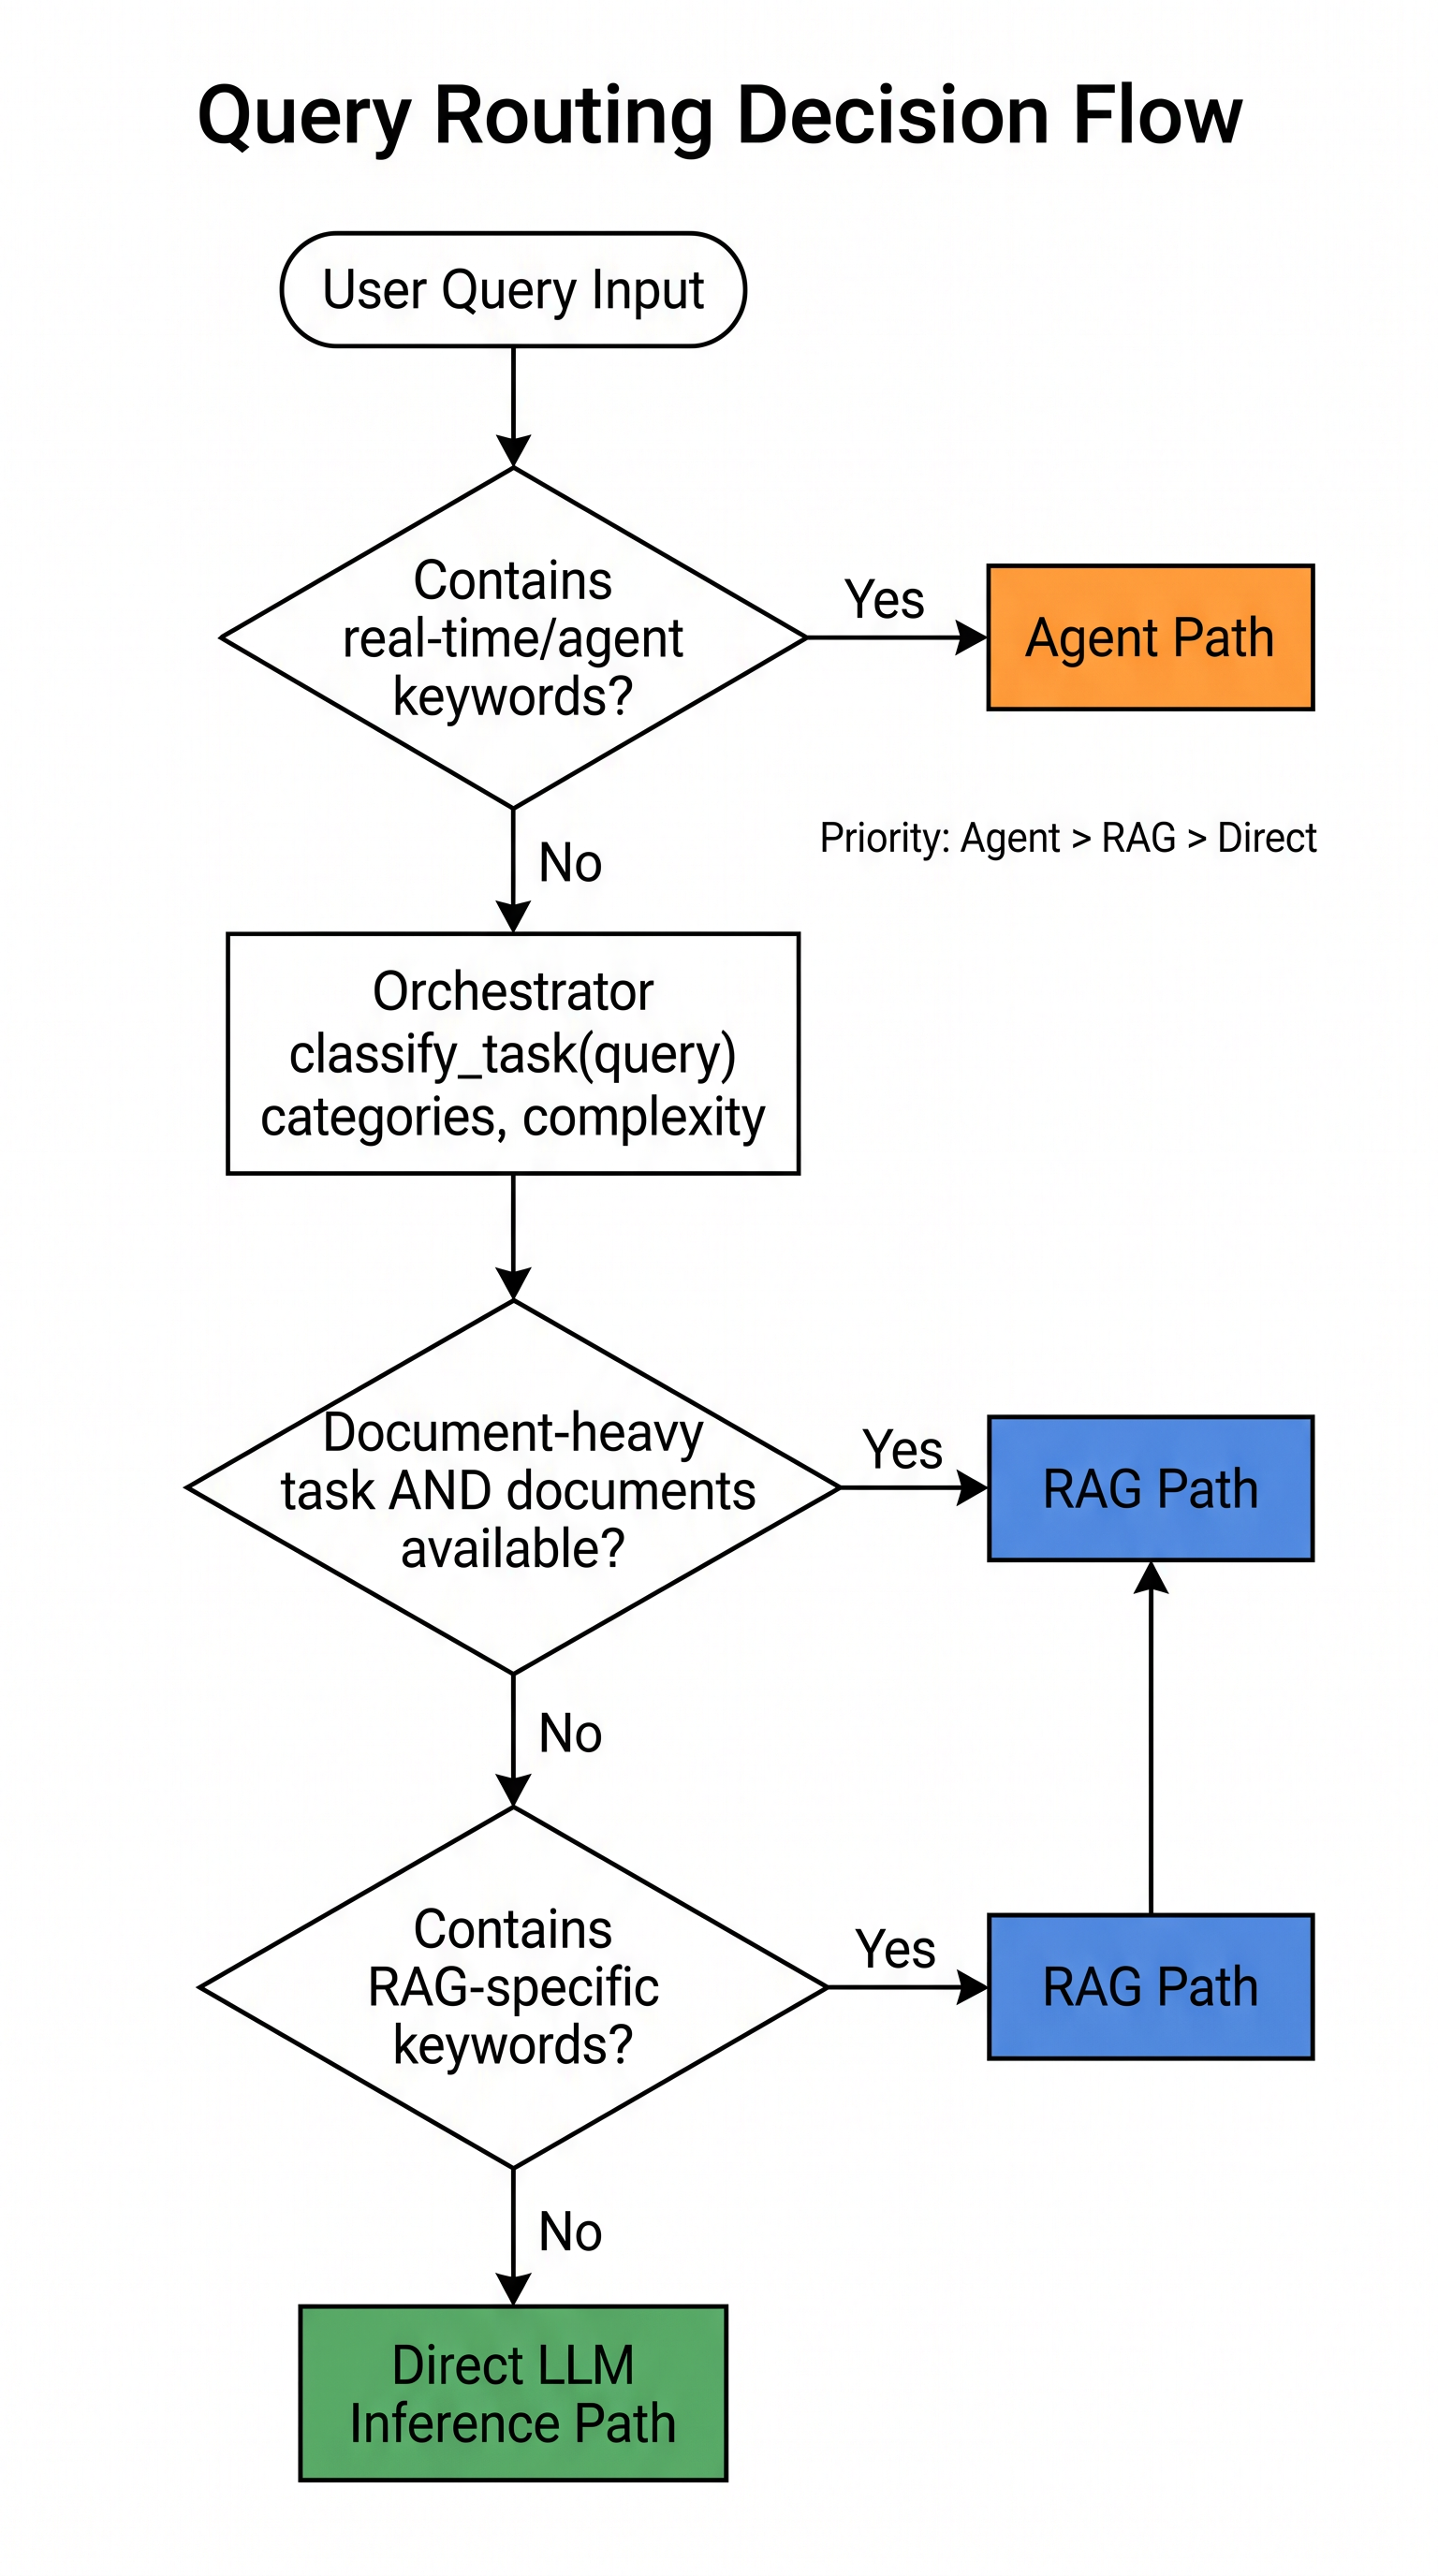
\includegraphics[height=0.7\linewidth]{../assets/query_routing.png}
    \caption{Query routing decision flowchart for the adaptive multi-path execution architecture.}
    \label{fig:routing_flow}
\end{figure}


\subsection{Direct Inference Node}
\label{subsec:direct_node}

The \texttt{direct\_node} handles queries that can be answered from parametric model knowledge without 
retrieval or agentic execution. It invokes the orchestrator's \\ \texttt{\_call\_llm\_with\_orchestrator} function, which performs task classification, model selection, specialist prompt construction, LLM invocation, optional synthesis, and attribution footer generation. The conversation history is trimmed to fit within the selected model's token limit before being injected into the prompt, preventing context overflow for long-running conversations.

\subsection{Retrieval-Augmented Generation Node}
\label{subsec:rag_node}

The \texttt{rag\_node} is activated when the router determines that document context is required. It first retrieves the top-$K$ relevant document chunks from a ChromaDB vector store through similarity search, where $K = 4$ by default. The retrieved chunks are concatenated into a \texttt{rag\_context} string that is prepended to the orchestrator prompt, instructing the model to ground its response in the provided evidence. The embedding function is provided by a sentence-transformer model deployed locally.

\begin{figure}[htbp]
    \centering
    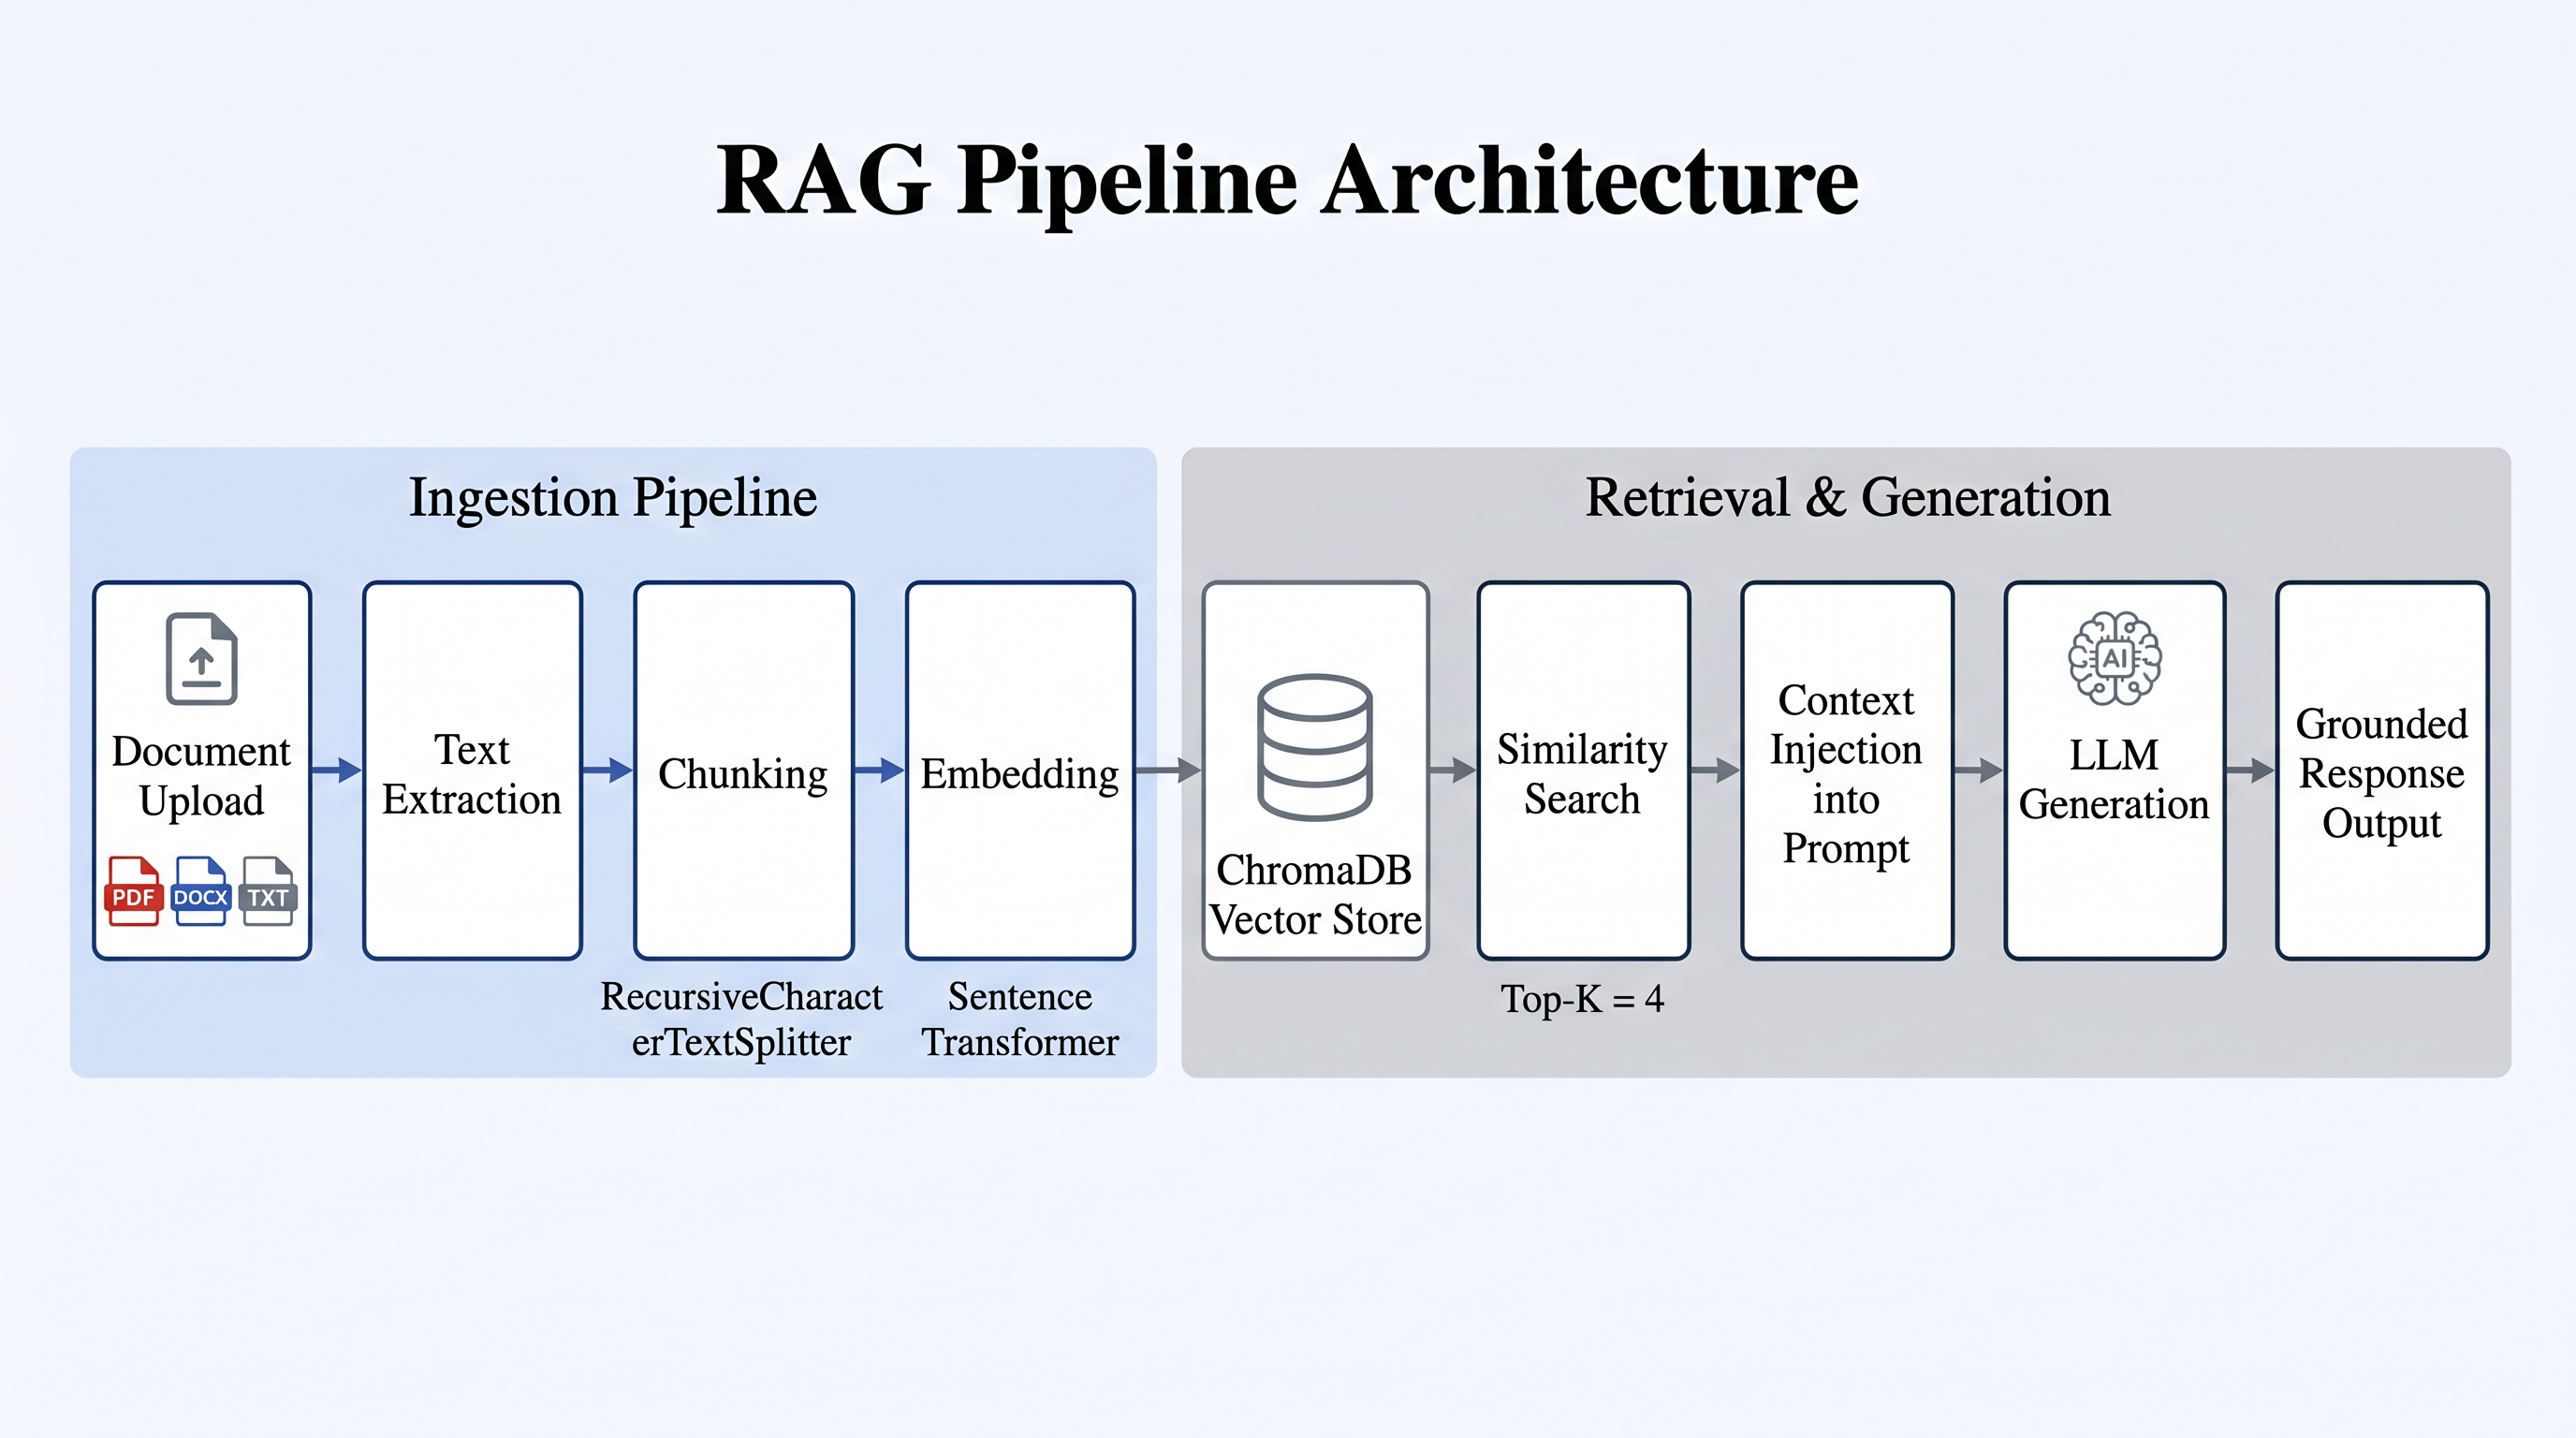
\includegraphics[width=0.9\linewidth]{../assets/rag_pipeline.png}
    \caption{RAG pipeline showing document ingestion, embedding, retrieval, and context injection.}
    \label{fig:rag_pipeline}
\end{figure}

The RAG ingestion pipeline, implemented in \texttt{app/rag/ingestion.py}, supports multiple document formats including PDF, DOCX, and plain text. Documents are split using LangChain's \texttt{RecursiveCharacterTextSplitter} with a configurable chunk size and overlap, and stored as embeddings in a persistent ChromaDB collection. The \texttt{get\_vectorstore\_count} function is called by the router to determine whether any documents are available before routing to the RAG path, preventing retrieval attempts on an empty collection.

\subsection{Agentic Execution Node}
\label{subsec:agent_node}

The \texttt{agent\_node} handles queries that require access to real-time information or computational capabilities beyond the model's parametric knowledge. The agent is equipped with two tools: a DuckDuckGo web search tool for retrieving current information, and a Python REPL calculator for performing mathematical computations. The agent executes in a ReAct-style loop, generating a chain of thought that interleaves reasoning steps with tool invocation decisions, continuing until the agent determines it has sufficient information to produce the final answer. The procedure is formalised in Algorithm~\ref{alg:agent}.


% ============================================================================
% Algorithm 4 – agent\_node (ReAct Execution)
% ============================================================================
\begin{algorithm}[H]
\caption{Agent node implementation showing ReAct-style execution with tool integration.}
\label{alg:agent}
\begin{algorithmic}[1]
\Procedure{AgentNode}{\ty{state}: ChatState} $\to$ dict
  \State $\ty{query}     \gets \Call{GetUserMessage}{\ty{state}}$
  \State $\ty{model\_key} \gets \ty{state.model}$ \textbf{ or } \ty{DEFAULT\_MODEL\_KEY}
 
  \State
  \State \cmt{Define tools available to the agent}
  \State $\ty{tools} \gets [\,\ty{DuckDuckGoSearchRun()},\ \ty{PythonREPLTool()}\,]$
 
  \State
  \State \cmt{Build ReAct agent with orchestrator-selected model}
  \State $\ty{llm}            \gets \Call{BuildLLM}{\ty{model\_key}}$
  \State $\ty{agent\_exec}    \gets \Call{CreateReActAgent}{\ty{llm},\, \ty{tools}}$
 
  \State
  \State \cmt{Execute agent with full conversation history as context}
  \State $\ty{history}        \gets \Call{BuildHistoryBlock}{\ty{state.messages},\, \ty{model\_key}}$
  \State $\ty{full\_prompt}   \gets \ty{history} + \texttt{"\textbackslash n\textbackslash nUser: "} + \ty{query}$
  \State $\ty{result}         \gets \Call{AgentExec.Invoke}{\{\ \ty{"messages"}: [(\ty{"user"},\, \ty{full\_prompt})]\ \}}$
  \State $\ty{response}       \gets \ty{result["messages"][-1].content}$
 
  \State
  \State \Return $\{\ \ty{messages}: [\Call{AIMessage}{\ty{response}}],\ \ty{rag\_context}: \ty{None},\ \ty{routing\_info}: \{\ty{model\_key},\ \ty{route}: \ty{"agent"}\}\ \}$
\EndProcedure
\end{algorithmic}
\end{algorithm}

Algorithm~\ref{alg:agent} details the sequential steps of the agentic execution procedure. The node first extracts the current user query from the shared state and resolves the active model key, falling back to \texttt{DEFAULT\_MODEL\_KEY} if none has been set. The tool suite is then instantiated, comprising \texttt{DuckDuckGoSearchRun} for live web retrieval and \texttt{PythonREPLTool} for arithmetic and computational tasks. An LLM instance is constructed from the resolved model key and passed alongside the tool suite to \texttt{CreateReActAgent}, which configures the ReAct-style reasoning loop. Prior to invocation, the full conversation history is serialised into a context block and prepended to the current query, ensuring the agent reasons over the complete dialogue context rather than the isolated turn. The agent executor is then invoked, internally iterating over thought--action--observation cycles until a terminal answer is produced. The final message in the output sequence is extracted as the response and returned to the shared state alongside routing metadata, with \texttt{rag\_context} explicitly set to \texttt{None} to signal that no retrieval was performed on this path.


\subsection{Persistence Layer: MySQL Checkpointing}
\label{subsec:persistence}

A critical feature of the system is persistent conversation management through a custom \texttt{MySQLSaver} class that implements LangGraph's \texttt{BaseCheckpointSaver} interface. Unlike the default in-memory saver, the MySQL-backed implementation persists conversation state across server restarts and supports multiple concurrent users through thread-local connection management. The checkpointer stores serialised \texttt{ChatState} snapshots keyed by thread ID and checkpoint ID, enabling exact state restoration for any conversation at any point in its history.

The \texttt{MySQLSaver} implements the \texttt{get\_tuple}, \texttt{list}, \texttt{put}, and \texttt{put\_writes} methods required by the LangGraph checkpointer interface, using \texttt{pymysql} for database connectivity with automatic reconnection on connection loss. A separate \texttt{delete\_thread} method enables users to delete conversation threads from both the in-memory session state and the persistent database.


\subsection{User Interface: Streamlit Application}
\label{subsec:ui}

The web-based user interface is implemented using Streamlit, providing a responsive chat interface with real-time streaming response display. The UI is organised into two primary components: a collapsible sidebar and a main chat area, each serving a distinct functional role within the overall system interaction model.

\subsubsection*{Sidebar Panel}
The sidebar, illustrated in Figure~\ref{fig:ui_sidebar}, serves as the primary control surface for session configuration and document management. At the top, the branding header displays the application identity — \textit{Zephryel, An AI Companion} — accompanied by a light/dark theme toggle for user preference persistence. Beneath the branding, the \textbf{Model} section exposes a dropdown selector that allows the user to either manually choose a specific language model from the deployed pool or delegate the decision to the system by selecting \textit{Auto (Multi-Model Routing)}, which activates the full orchestrator-driven routing pipeline. A contextual label beneath the dropdown indicates the active inference provider, confirming that all inference is served through Groq's API. The \textbf{Conversations} section provides thread management functionality, including a prominently placed \textit{New Chat} button that initialises a fresh conversation thread with a unique identifier, alongside per-thread action controls for renaming and deletion. The \textbf{Documents (RAG)} section at the bottom of the sidebar presents the current state of the vector store, displaying the ChromaDB persistence path and the total number of indexed chunks currently available for retrieval. A drag-and-drop file uploader accepts PDF and TXT documents up to 200MB per file, triggering the ingestion pipeline upon upload to parse, chunk, embed, and index the document into the ChromaDB collection.

\begin{figure}[H]
    \centering
    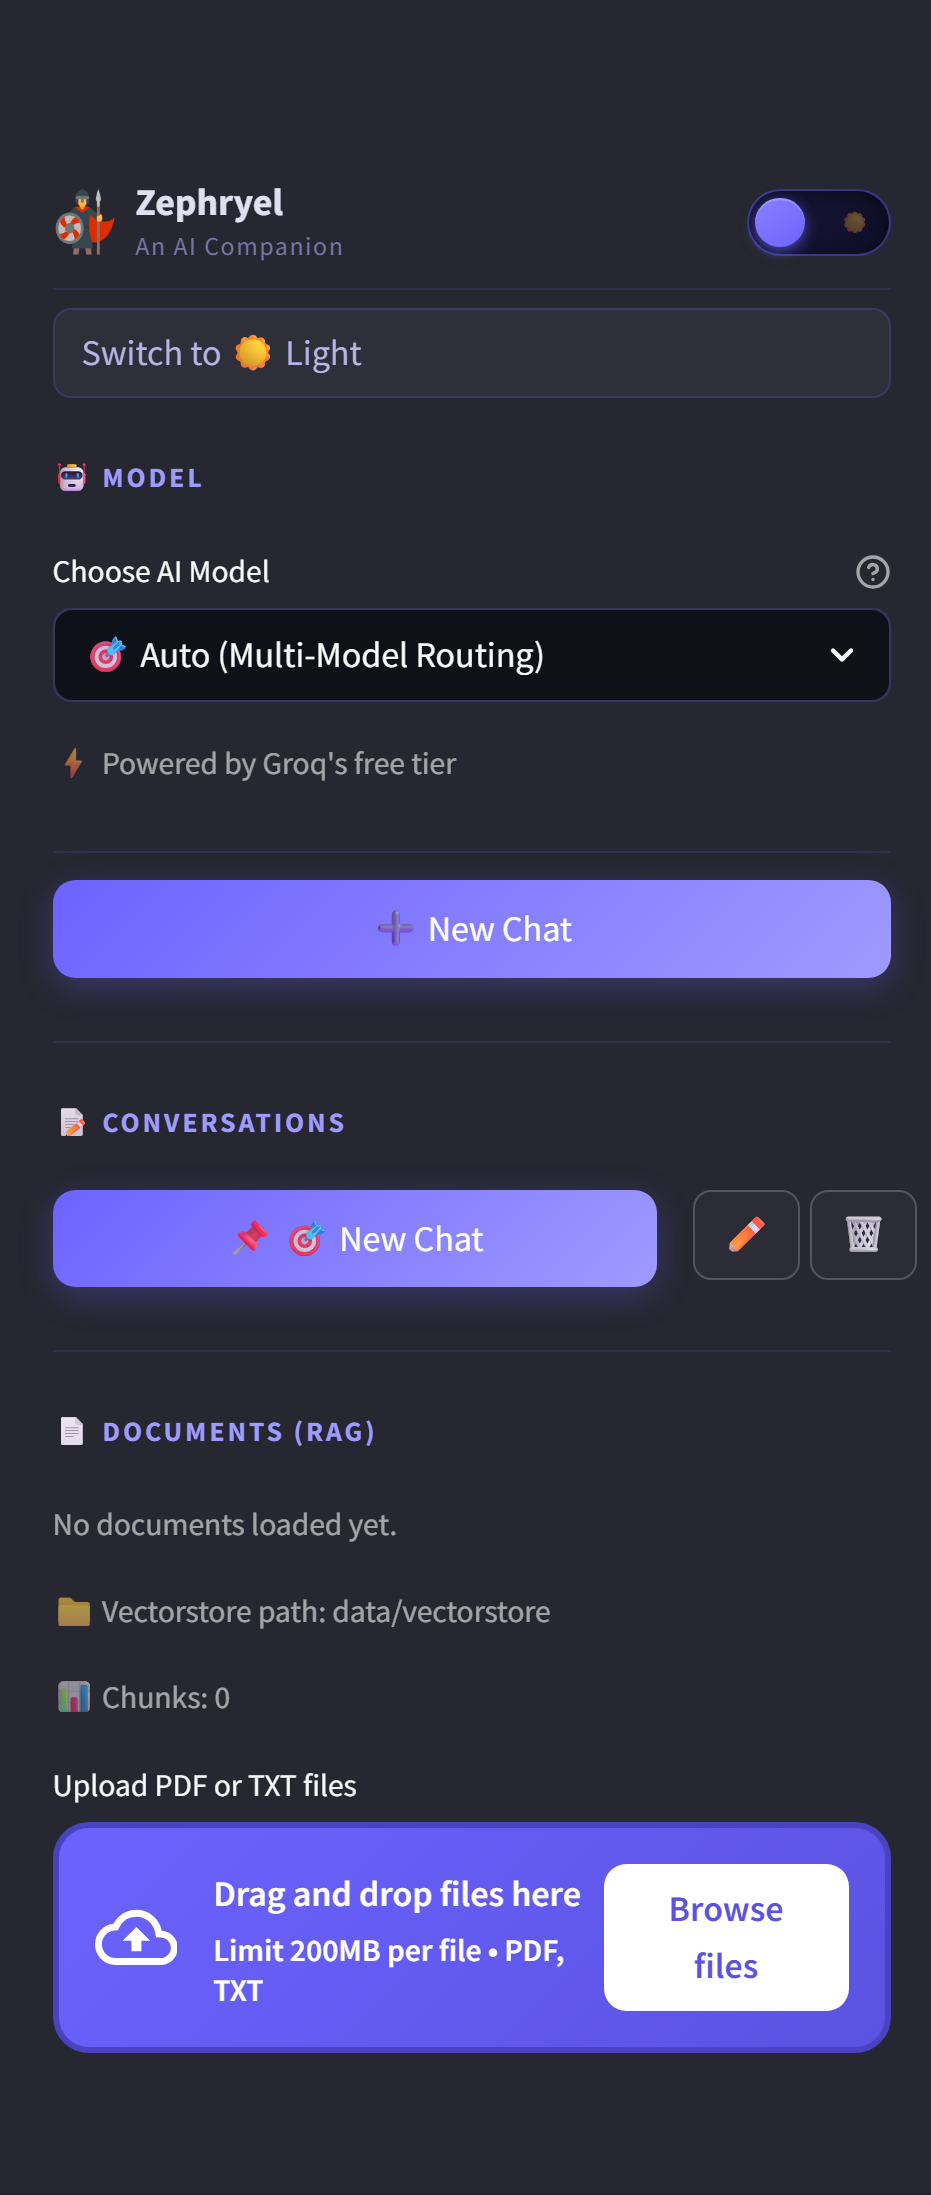
\includegraphics[
        height=0.7\linewidth,
        keepaspectratio
    ]{../assets/sidebar.png}
    \caption{Sidebar panel showing the model selector defaulting to Auto (Multi-Model Routing), conversation thread management controls, and the RAG document upload panel with ChromaDB vector store status.}
    \label{fig:ui_sidebar}
\end{figure}

\subsubsection*{Main Chat Area}
The main chat area, illustrated in Figure~\ref{fig:ui_chat}, provides the primary conversational interface. Each conversation turn is rendered with role-appropriate styling: user messages are displayed in a visually distinct bubble with a user avatar, while assistant responses are rendered with an assistant avatar and full markdown support, including bold emphasis, bullet points, code blocks, and inline formatting. The conversation title is auto-generated from the first user message using a lightweight title-generation prompt, providing meaningful thread labels in the sidebar. Streaming responses are rendered progressively using Streamlit's \texttt{st.write\_stream} interface, displaying partial tokens as they arrive from the Groq inference API to minimise perceived latency. Below each assistant response, a collapsible \textbf{Model Routing} metadata panel provides full transparency into the orchestrator's decision-making for that turn. As shown in Figure~\ref{fig:ui_chat}, the panel surfaces three key routing attributes: the inferred \textit{Task} category (e.g., \texttt{CONVERSATIONAL}, \texttt{REASONING}, \texttt{CODING}), the assessed \textit{Complexity} level (\texttt{LOW}, \texttt{MEDIUM}, or \texttt{HIGH}), and the \textit{Model} key of the specialist language model selected for that specific query. This routing transparency mechanism is a deliberate design choice to make the system's adaptive behaviour interpretable and auditable by the end user, distinguishing the interface from conventional single-model chatbot UIs where model selection is entirely opaque.

\begin{figure}[H]
    \centering
    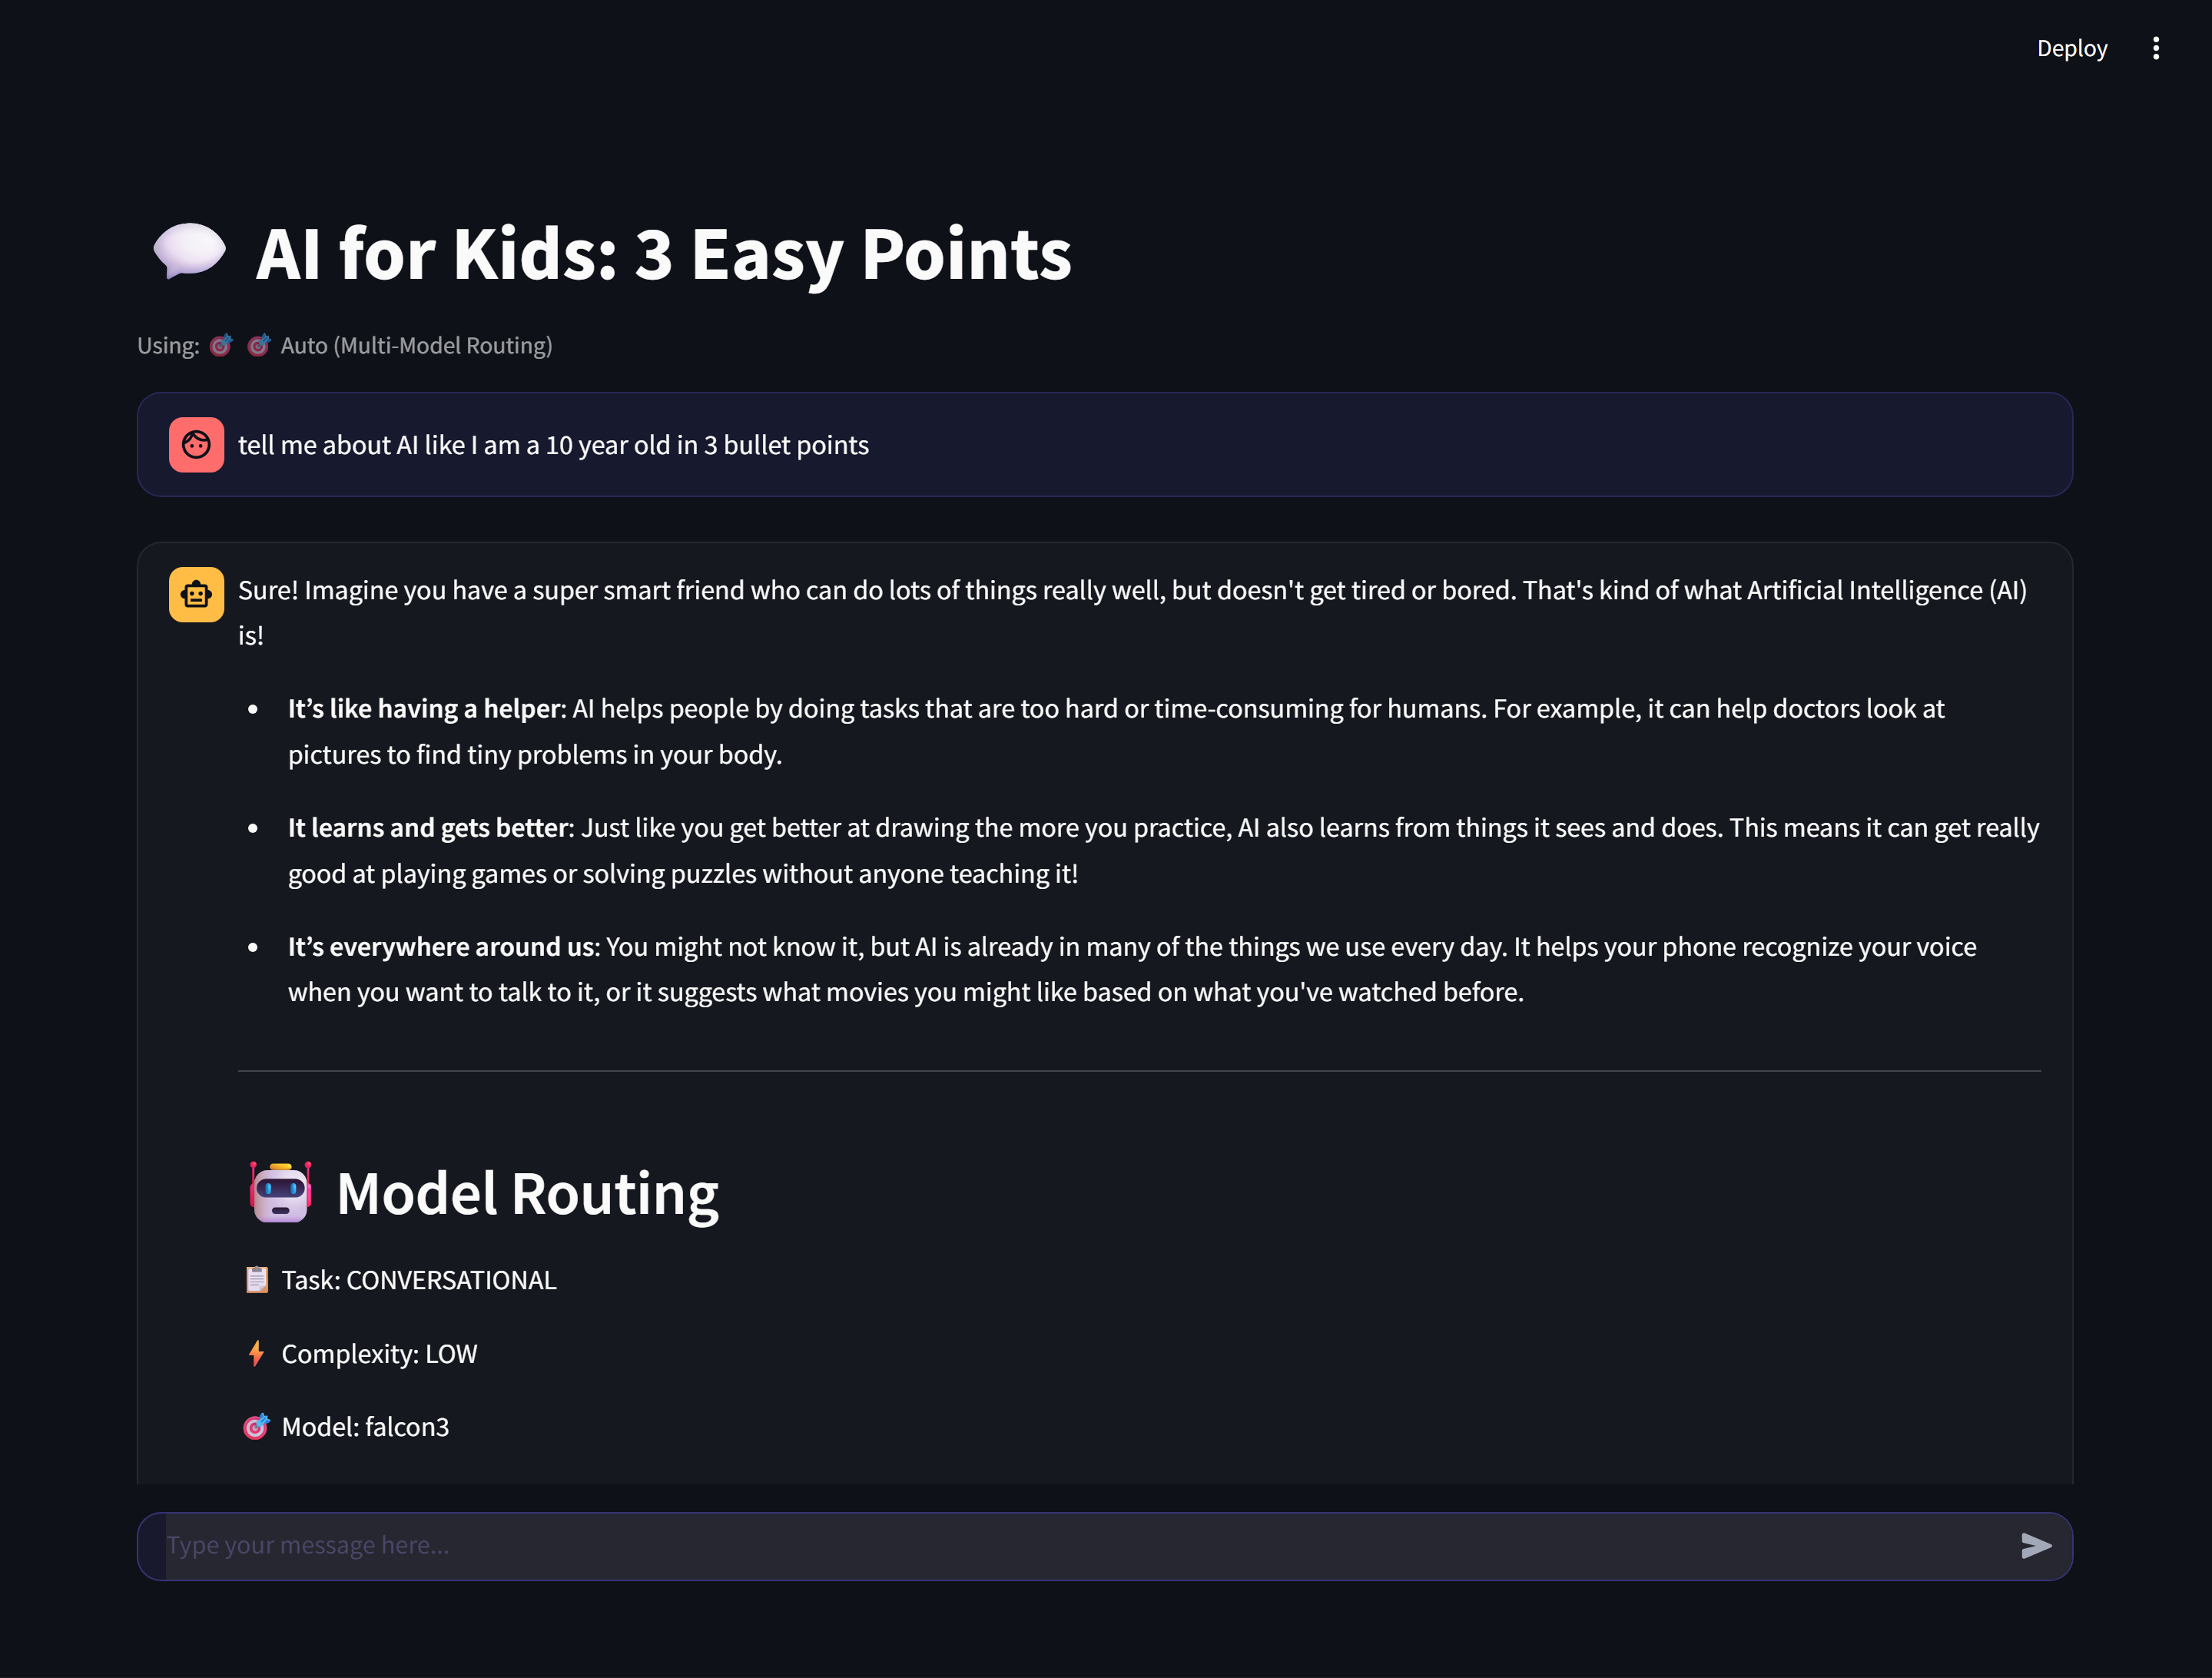
\includegraphics[
        width=0.9\linewidth,
        keepaspectratio
    ]{../assets/chat.png}
    \caption{Main chat area showing a multi-turn conversation with markdown-rendered assistant response and the Model Routing transparency panel displaying inferred task classification (\texttt{CONVERSATIONAL}), complexity (\texttt{LOW}), and the specialist model selected for the turn (\texttt{falcon3}).}
    \label{fig:ui_chat}
\end{figure}


\subsection{System Design Summary}
\label{subsec:design_summary}


The system design achieves several key properties that address the limitations identified in Section~\ref{sec:literature_review}. Selectivity is achieved through the routing mechanism that avoids unnecessary retrieval and agentic overhead. Specialist alignment is achieved through orchestrator-driven model selection that matches query type to model strengths. Persistence is provided through MySQL-backed state management. Extensibility is supported by the modular node-based architecture, where new models or execution paths can be added without modifying existing components.
\begin{figure}[htbp]
    \centering
    \includegraphics[width=0.9\linewidth]{../assets/graphical_abstract.png}
    \caption{LangGraph StateGraph topology showing nodes, conditional edges, and execution paths.}
    \label{fig:langgraph_topology}
\end{figure}

\newpage

% % =================================================

\section{Implementation}
\label{sec:implementation}

\subsection{Technology Stack}
\label{subsec:tech_stack}

The system is implemented in Python 3.12, selected for its extensive ecosystem of AI and NLP libraries and its strong support for asynchronous and concurrent programming patterns. The core dependencies are LangGraph 1.1.9 for stateful orchestration, LangChain 1.2.15 for LLM abstraction and tool integration, ChromaDB for vector storage, pymysql for MySQL connectivity, Streamlit for the web frontend, and the Groq Python SDK for accessing hosted LLM inference. The complete dependency set is specified in the project's \texttt{requirements.txt} and \texttt{pyproject.toml} files.

\subsection{Project Structure}
\label{subsec:project_structure}

The codebase is organised into a modular package structure designed for maintainability and testability, as shown in Listing~\ref{lst:structure}.

\begin{lstlisting}[caption={Project directory structure of the LangGraph chatbot implementation.}, label={lst:structure}, language=bash]
langgraph_chatbot/
├── api.py                    # FastAPI REST backend for Android app
├── main.py                   # Streamlit application entry point
├── app/
│   ├── core/
│   │   ├── graph.py          # Main LangGraph StateGraph and nodes
│   │   └── streaming.py      # Streaming response utilities
│   ├── models/
│   │   └── chat_state.py     # ChatState TypedDict schema
│   ├── rag/
│   │   ├── ingestion.py      # Document parsing and ChromaDB indexing
│   │   ├── retriever.py      # Similarity search and context retrieval
│   │   └── embedder.py       # Sentence-transformer embedding function
│   ├── ui/
│   │   ├── chat.py           # Message rendering and chat interface
│   │   └── sidebar.py        # Model selector, RAG panel, thread list
│   └── utils/
│       ├── thread_service.py # Thread CRUD and conversation management
│       └── conversation.py   # Message formatting utilities
├── config/
│   └── settings.py           # Environment and API key configuration
├── data/
│   └── vectorstore/          # Persistent ChromaDB vector store
└── llms/
    └── custom/
        └── orchestrator.py   # Task classification and model routing
\end{lstlisting}

\subsection{LLM Integration via Groq}
\label{subsec:groq_integration}

All LLM inference is performed through the Groq inference API, which provides low-latency access to open-weight models via a standardised OpenAI-compatible interface. The \texttt{llms.build\_llm(model\_key)} factory function constructs a LangChain-compatible LLM wrapper for the specified model key, handling API authentication, model name resolution, and parameter configuration. Token limit management is implemented through the \texttt{\_trim\_messages} function, which truncates conversation history to fit within each model's context window while preserving the most recent turns. The factory pattern is formalised in Algorithm~\ref{alg:build_llm}.


% ============================================================================
% Algorithm 5 – build\_llm (LLM Factory)
% ============================================================================

\begin{algorithm}[H]
\caption{LLM factory function mapping model keys to Groq-hosted model instances.}
\label{alg:build_llm}
\begin{algorithmic}[1]
  \State \cmt{MODEL\_REGISTRY: internal key $\mapsto$ Groq model identifier}
  \State $\text{MODEL\_REGISTRY} \gets$
  \State \hspace{\algorithmicindent}
    $\{$
    \ty{"deepseek\_r1"} $\mapsto$ \ty{"deepseek-r1-distill-llama-70b"},
  \State \hspace{\algorithmicindent}
    \ty{"falcon3"} $\mapsto$ \ty{"falcon-3-10b-instruct"},
  \State \hspace{\algorithmicindent}
    \ty{"gemini\_2\_5\_flash"} $\mapsto$ \ty{"gemma2-9b-it"},
  \State \hspace{\algorithmicindent}
    \ty{"gemma3\_270m"} $\mapsto$ \ty{"gemma-7b-it"},
  \State \hspace{\algorithmicindent}
    \ty{"granite3\_dense\_2b"} $\mapsto$ \ty{"llama-3.1-8b-instant"},
  \State \hspace{\algorithmicindent}
    \ty{"llama\_3\_1\_8b\_instant"} $\mapsto$ \ty{"llama-3.1-8b-instant"},
  \State \hspace{\algorithmicindent}
    \ty{"mistral\_7b"} $\mapsto$ \ty{"mixtral-8x7b-32768"},
  \State \hspace{\algorithmicindent}
    \ty{"phi3\_3\_8b"} $\mapsto$ \ty{"llama3-8b-8192"},
  \State \hspace{\algorithmicindent}
    \ty{"qwen2\_5\_coder\_7b"} $\mapsto$ \ty{"qwen-qwq-32b"},
  \State \hspace{\algorithmicindent}
    \ty{"qwen3\_5\_0\_8b"} $\mapsto$ \ty{"llama-3.2-1b-preview"}
    $\}$
\Function{BuildLLM}{\ty{model\_key}: str} $\to$ BaseChatModel
  \State $\ty{model\_name} \gets \text{MODEL\_REGISTRY}\!\left[\ty{model\_key}\right]$
  \State \Return $\Call{ChatGroq}{\ty{model}=\ty{model\_name},\ \ty{temperature}=0.7,\ \ty{api\_key}=\ty{settings.GROQ\_API\_KEY}}$
\EndFunction
\end{algorithmic}
\end{algorithm}

Algorithm~\ref{alg:build_llm} defines two components. The first is \texttt{MODEL\_REGISTRY}, a static mapping from the system's internal model keys to their corresponding Groq-hosted model identifiers. Several entries in this registry reflect deployment constraints: for instance, \texttt{gemini\_2\_5\_flash} resolves to \texttt{gemma2-9b-it} and \texttt{qwen2\_5\_coder\_7b} resolves to \texttt{qwen-qwq-32b}, as these represent the closest available Groq-hosted equivalents at the time of deployment. Lightweight keys such as \texttt{qwen3\_5\_0\_8b} map to compact preview models, while the default fallback \texttt{llama\_3\_1\_8b\_instant} and \texttt{granite3\_dense\_2b} both resolve to \texttt{llama-3.1-8b-instant}, prioritising availability and latency. The second component is the \texttt{BuildLLM} function itself, which performs a single registry lookup on the provided key and constructs a \texttt{ChatGroq} instance with a fixed temperature of $0.7$ and the globally configured API key, returning a \texttt{BaseChatModel} compatible with the LangChain execution environment.


\subsection{RAG Document Ingestion Pipeline}
\label{subsec:rag_implementation}

The RAG ingestion pipeline processes user-uploaded documents through a three-stage pipeline: parsing, chunking, and embedding. The parsing stage supports PDF (via PyPDF2), DOCX (via python-docx), and plain text formats. Parsed text is split using LangChain's \texttt{RecursiveCharacterTextSplitter} with a chunk size of 1,000 characters and 200-character overlap, balancing retrieval precision with context sufficiency. Chunks are embedded using a sentence-transformer model and stored in a persistent ChromaDB collection. The complete ingestion procedure is formalised in Algorithm~\ref{alg:ingestion}.


% ============================================================================
% Algorithm – ingest\_documents (RAG Ingestion Pipeline)
% ============================================================================
\begin{algorithm}[H]
\caption{Document ingestion pipeline showing chunking and ChromaDB indexing}
\label{alg:ingestion}
\begin{algorithmic}[1]
\Function{IngestDocuments}{\ty{file\_paths}: list[str]} $\rightarrow$ int

  \State $\ty{splitter} \gets \text{RecursiveCharacterTextSplitter}()$
  \State \hspace{\algorithmicindent} $\ty{chunk\_size} = 1000$,
  \State \hspace{\algorithmicindent} $\ty{chunk\_overlap} = 200$,
  \State \hspace{\algorithmicindent} $\ty{separators} = [\texttt{"\textbackslash n\textbackslash n"}, \texttt{"\textbackslash n"}, \texttt{" "}, \texttt{""}]$

  \State $\ty{all\_chunks} \gets [\ ]$

  \For{each $\ty{path} \in \ty{file\_paths}$}
    \State $\ty{text}   \gets \text{ParseDocument}(\ty{path})$
    \State $\ty{chunks} \gets \ty{splitter}.\text{CreateDocuments}(\ty{text},\ \ty{path})$
    \State $\ty{all\_chunks} \gets \ty{all\_chunks} + \ty{chunks}$
  \EndFor

  \State \cmt{Embed and store in persistent ChromaDB collection}
  \State $\ty{vs} \gets \text{Chroma}.\text{FromDocuments}(\ty{all\_chunks},\ \text{GetEmbedder}())$
  \State $\ty{vs}.\ty{collection\_name}   \gets \ty{COLLECTION\_NAME}$
  \State $\ty{vs}.\ty{persist\_directory} \gets \ty{VECTORSTORE\_DIR}$

  \State \Return $|\ty{all\_chunks}|$
\EndFunction
\end{algorithmic}
\end{algorithm}

Algorithm~\ref{alg:ingestion} proceeds in three phases. In the initialisation phase, a \\ \texttt{RecursiveCharacterTextSplitter} is configured with a chunk size of 1,000 characters and an overlap of 200 characters. The separator hierarchy — paragraph breaks, line breaks, spaces, and the empty string — ensures that splits are attempted at the most semantically natural boundary available before falling back to finer granularities, preventing context loss at chunk boundaries. In the parsing and chunking phase, each file path is dispatched through \texttt{ParseDocument}, which routes to the appropriate parser based on file format, producing a raw text string. This text is then passed to the splitter's \texttt{CreateDocuments} method, which attaches the source path as document metadata before appending the resulting chunks to the accumulated list. In the final indexing phase, all collected chunks are embedded in a single batch via \texttt{Chroma.FromDocuments}, which internally calls \texttt{GetEmbedder} to obtain the sentence-transformer model. The resulting vector store is bound to the configured collection name and persistence directory, ensuring the index survives across sessions. The function returns the total number of chunks indexed, providing a lightweight confirmation of ingestion volume.



\subsection{Conversation Thread Management}
\label{subsec:thread_management}

Each conversation is identified by a unique thread ID generated at session creation time. The \texttt{thread\_service.py} module provides CRUD operations for thread management, including creation, retrieval, title generation, and deletion. Thread titles are auto-generated by passing the first user message to a lightweight LLM with a title-generation prompt, providing meaningful conversation labels in the sidebar. The thread service interfaces with both the MySQL checkpointer (for state persistence) and Streamlit session state (for UI synchronisation).

\subsection{Streaming Responses}
\label{subsec:streaming}

Response streaming is implemented through LangGraph's event streaming API, which yields partial response tokens as they are generated by the LLM. The \texttt{streaming.py} module wraps the graph's \texttt{astream\_events} method, filtering for \texttt{on\_chat\_model\_stream} events to extract token deltas. The Streamlit frontend uses an \texttt{st.write\_stream} call to render tokens progressively, providing a responsive user experience that begins displaying content before the full response is complete.

\subsection{FastAPI REST Backend}
\label{subsec:api}

The \texttt{api.py} module implements a FastAPI REST backend that exposes the full chatbot functionality as HTTP endpoints, primarily for consumption by the Android mobile application. The available endpoints are formalised in Algorithm~\ref{alg:api}.

% ============================================================================
% Algorithm 7 – FastAPI REST Endpoints
% ============================================================================
\begin{algorithm}[H]
\caption{FastAPI REST endpoint definitions for the Android application backend.}
\label{alg:api}
\begin{algorithmic}[1]
  \State \cmt{--- \textbf{POST} \ty{/chat} ---}
\Procedure{Chat}{\ty{request}: ChatRequest} $\to$ ChatResponse
\EndProcedure
 
\vspace{4pt}
  \State \cmt{--- \textbf{GET} \ty{/threads} ---}
\Procedure{ListThreads}{\ty{user\_id}: str} $\to$ list[ThreadMeta]
\EndProcedure
 
\vspace{4pt}
  \State \cmt{--- \textbf{POST} \ty{/threads} ---}
\Procedure{CreateThread}{\ty{user\_id}: str} $\to$ ThreadMeta
\EndProcedure
 
\vspace{4pt}
  \State \cmt{--- \textbf{DELETE} \ty{/threads/\{thread\_id\}} ---}
\Procedure{DeleteThread}{\ty{thread\_id}: str} $\to$ dict
\EndProcedure
 
\vspace{4pt}
  \State \cmt{--- \textbf{POST} \ty{/rag/upload} ---}
\Procedure{UploadDocument}{\ty{file}: UploadFile} $\to$ dict
\EndProcedure
\end{algorithmic}
\end{algorithm}

Algorithm~\ref{alg:api} defines five endpoints. The \texttt{POST /chat} endpoint is the primary entry point, accepting a \texttt{ChatRequest} payload and routing it through the full LangGraph pipeline before returning a \texttt{ChatResponse} containing the model's reply and associated routing metadata. The \texttt{GET /threads} endpoint retrieves the list of all conversation threads associated with a given user identifier, returning a collection of \texttt{ThreadMeta} descriptors. The \texttt{POST /threads} endpoint creates a new conversation thread for the specified user, returning the newly created \texttt{ThreadMeta}. The \texttt{DELETE /threads/\{thread\_id\}} endpoint removes the specified thread and its associated history from the persistent store. Finally, the \texttt{POST /rag/upload} endpoint accepts a multipart file upload and dispatches it through the document ingestion pipeline described in Section~\ref{subsec:rag_implementation}, indexing the content into the ChromaDB vector store for subsequent retrieval.

The API is designed for stateless horizontal scalability; all state is managed through the MySQL checkpointer, allowing multiple API server instances to serve the same users concurrently.

\FloatBarrier

\newpage




\section{Android Application}
\label{sec:android}

\subsection{Overview}
\label{subsec:android_overview}

To extend the adaptive multi-LLM chatbot system to mobile users, a companion Android application was developed that mirrors the core functionality of the Streamlit web interface. The application communicates with the FastAPI REST backend described in Section~\ref{subsec:api}, utilizing the same LangGraph-based orchestration, model routing, RAG pipeline, and persistent conversation handling. The application targets API level 26 (Android 8.0) and above.

\subsection{Mobile Dashboard}
\label{subsec:android_dashboard}

\begin{figure}[htbp]
    \centering
    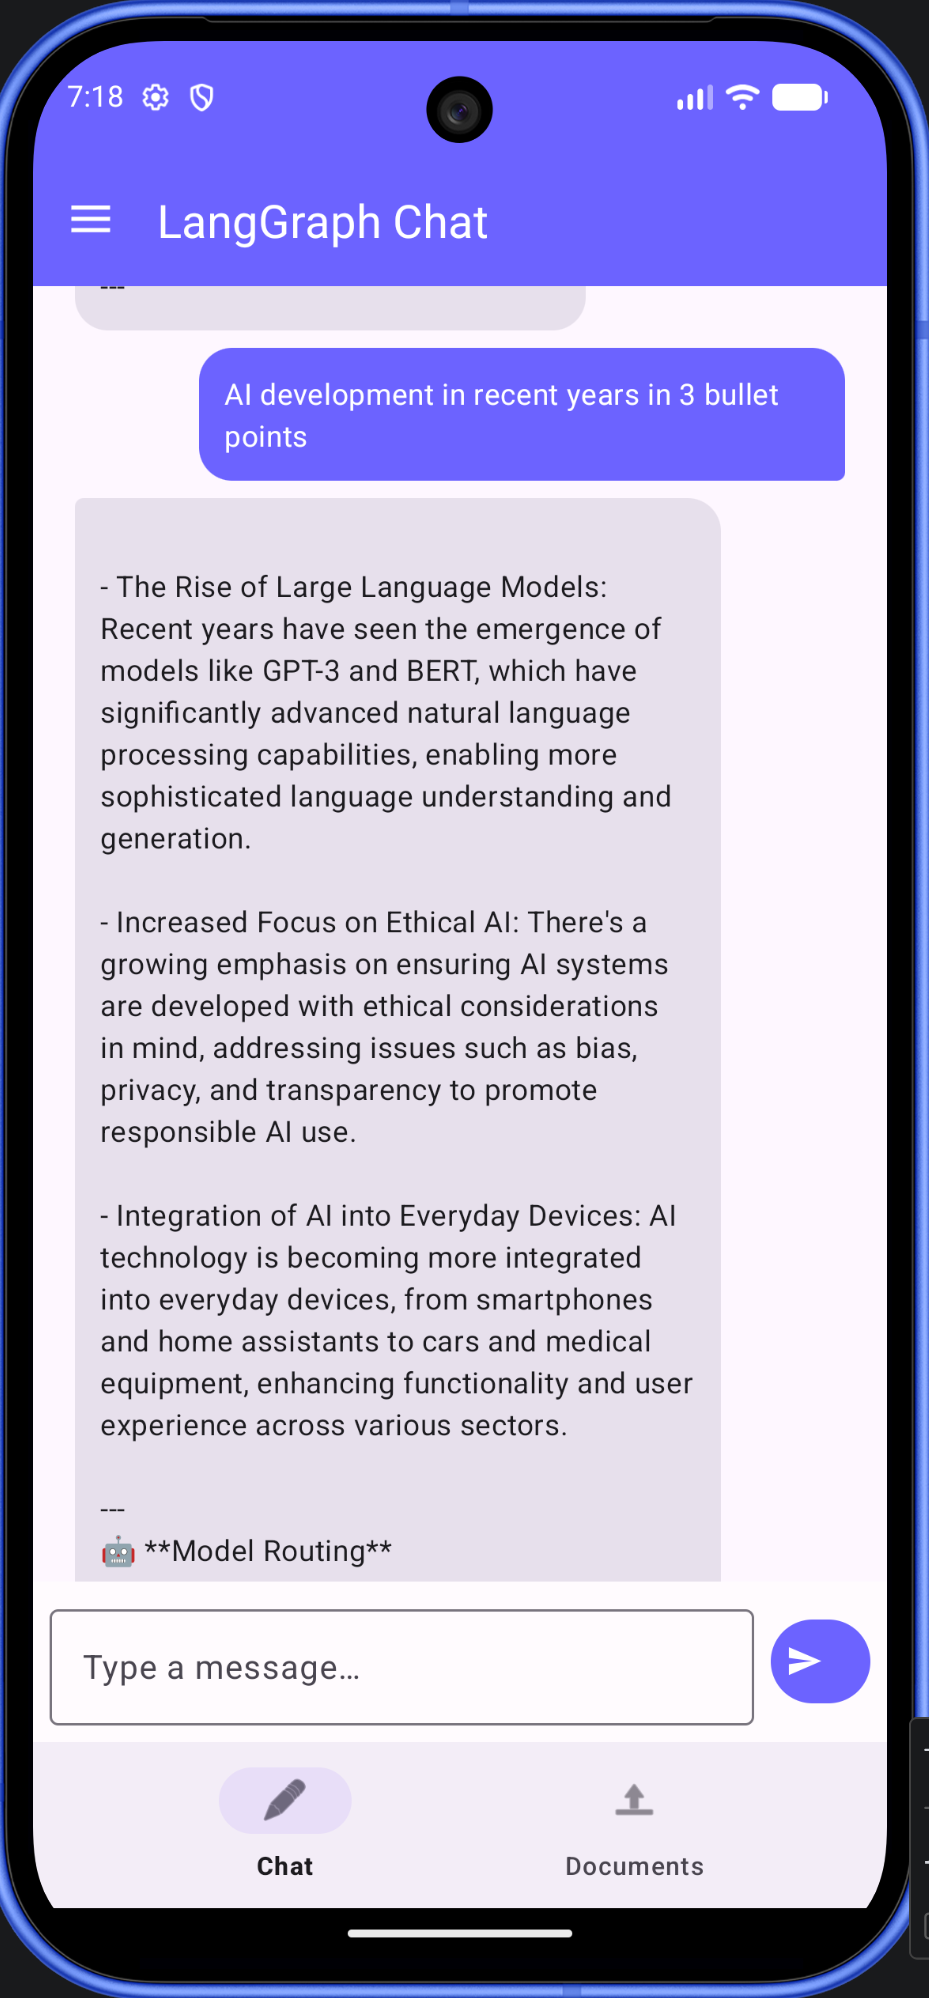
\includegraphics[height=0.7\linewidth]{../assets/mobile_dashboard.png}
    \caption{Mobile dashboard of the Android application showing chat interface, model interaction, and routing transparency.}
    \label{fig:mobile_dashboard}
\end{figure}

The mobile dashboard presents the primary user interface of the application. It includes a real-time chat interface with structured message bubbles, a user input field with a send action, and integrated routing transparency indicating model selection behavior. The interface is designed using Jetpack Compose to ensure responsiveness and a modern user experience.

\subsection{Key Features}
\label{subsec:android_features}

The application provides a streamlined set of features. The Chat Interface enables real-time conversations with dynamic message rendering. The Model Selection mechanism allows users to either manually select a model or rely on automatic routing. The Thread Management system supports retrieval and continuation of past conversations. The Document Upload functionality enables users to upload files for retrieval-augmented generation. Additionally, routing transparency is displayed to inform users about model decisions.

\subsection{Interaction Flow}
\label{subsec:android_flow}

\begin{figure}[htbp]
    \centering
    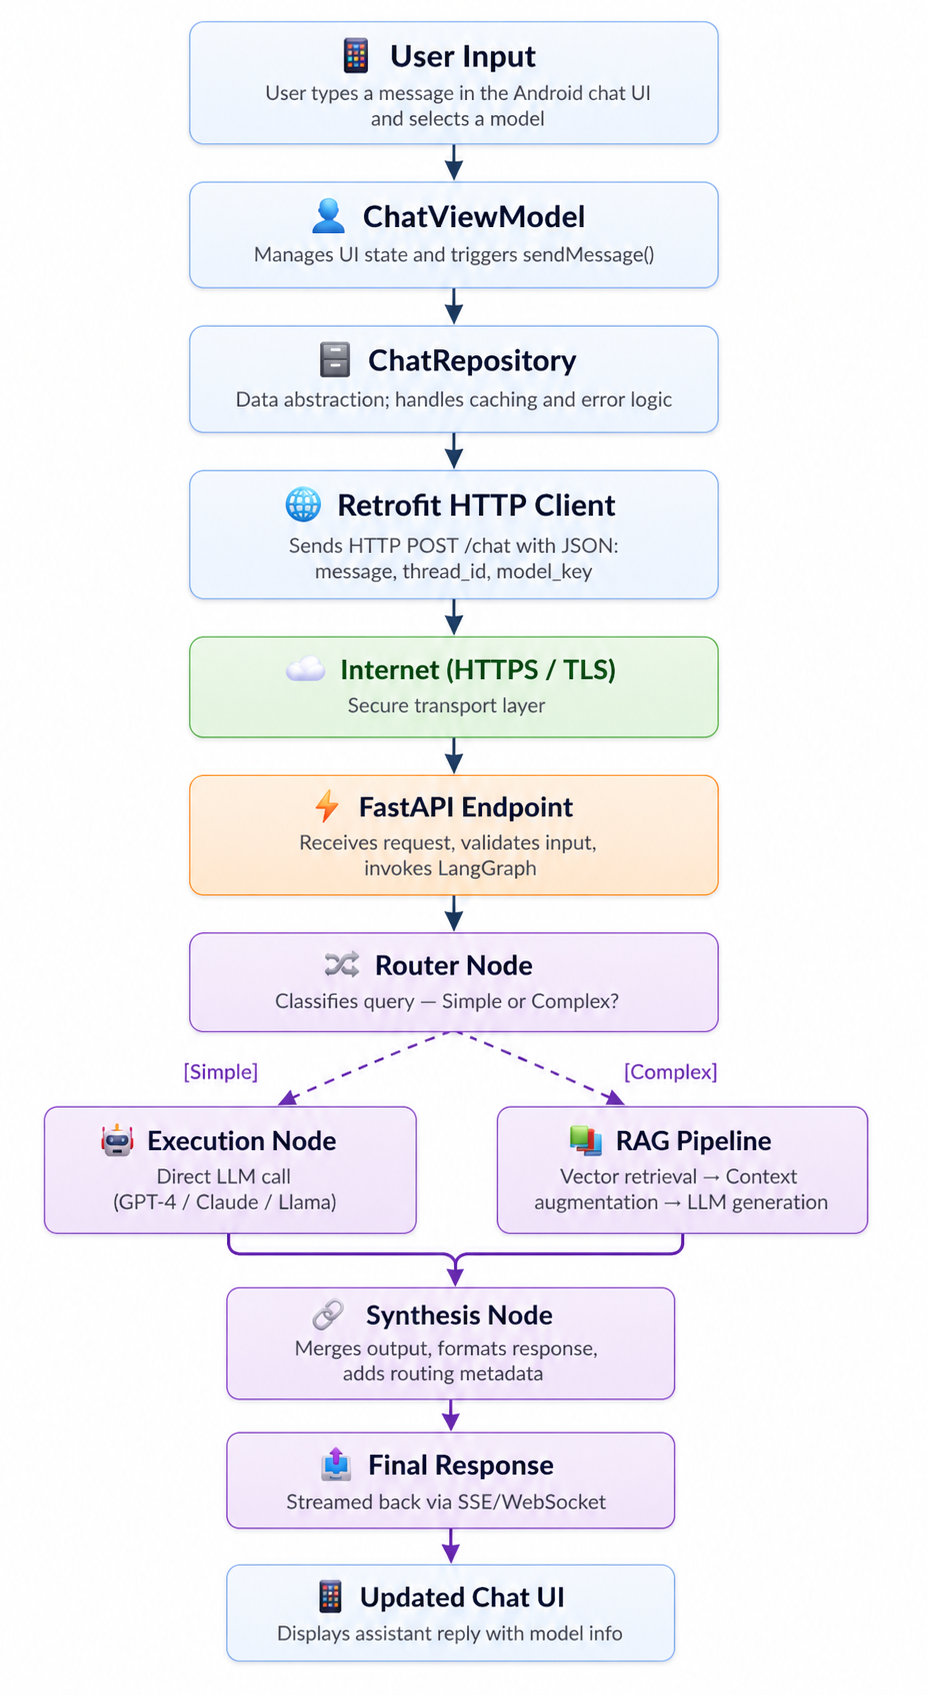
\includegraphics[height=0.7\linewidth]{../assets/android_flowchart.png}
    \caption{End-to-End Interaction Flow of Android-based Multi-LLM Chatbot System}
    \label{fig:mobile_flowchart}
\end{figure}

The interaction begins when a user submits a message through the chat interface. The request is handled by the ViewModel and sent via the repository layer to the FastAPI backend using an HTTP POST request. The backend processes the request through the LangGraph pipeline, performing routing and execution. The generated response is returned to the application, where the UI state is updated and rendered dynamically in the chat interface.

\newpage

\section{Results}
\label{sec:results}

\subsection{Experimental Setup}
\label{subsec:eval_setup}

The system is evaluated on two multi-hop question-answering benchmark
datasets: HotpotQA~(Yang et al., 2018) and MuSiQue~(Trivedi et al., 2022).
For each dataset, 500 questions are evaluated.
Metrics include Exact Match (EM), Token-level F1, Retrieval
Precision@4, and average latency.
All experiments use Groq-hosted inference with temperature~0.7.

% ── HotpotQA ─────────────────────────────────────────────────────────
\subsection{HotpotQA Results}
\label{subsec:hotpotqa_results}

Table~\ref{tab:hotpotqa} presents the evaluation results on the
HotpotQA benchmark.

\begin{table}[htbp]
  \centering
  \caption{Model performance on HotpotQA (500 questions).}
  \label{tab:hotpotqa}
  \begin{tabular}{lcccc}
    \hline
    \textbf{Model}
      & \textbf{EM (\%)}
      & \textbf{F1 (\%)}
      & \textbf{Retrieval P@4}
      & \textbf{Lat (ms)} \\
    \hline
    DeepSeek-R1            & 70.2 & 75.8 & 0.865 & 3850 \\
    Falcon3                & 36.5 & 42.1 & 0.723 &  215 \\
    Gemini-2.5-Flash       & 65.4 & 71.2 & 0.854 &  520 \\
    Gemma3-270M            & 18.2 & 23.5 & 0.512 &   78 \\
    Granite3-Dense-2B      & 28.7 & 34.3 & 0.642 &  142 \\
    LLaMA-3.1-8B-Instant   & 58.3 & 63.9 & 0.838 &  310 \\
    Mistral-7B             & 55.6 & 61.4 & 0.821 &  295 \\
    Phi3-3.8B              & 48.9 & 54.2 & 0.795 &  268 \\
    Qwen2.5-Coder-7B       & 60.1 & 66.5 & 0.846 &  305 \\
    Qwen3.5-0.8B           & 22.4 & 28.9 & 0.587 &  105 \\
    \hline
    \textbf{Adaptive (Ours)} & \textbf{62.5} & \textbf{68.3} & \textbf{0.875} & 485 \\
    \hline
  \end{tabular}
\end{table}

% ── MuSiQue ──────────────────────────────────────────────────────────
\subsection{MuSiQue Results}
\label{subsec:musique_results}

Table~\ref{tab:musique} presents the evaluation results on the
MuSiQue benchmark.

\begin{table}[htbp]
  \centering
  \caption{Model performance on MuSiQue (500 questions).}
  \label{tab:musique}
  \begin{tabular}{lcccc}
    \hline
    \textbf{Model}
      & \textbf{EM (\%)}
      & \textbf{F1 (\%)}
      & \textbf{Retrieval P@4}
      & \textbf{Lat (ms)} \\
    \hline
    DeepSeek-R1            & 55.1 & 59.3 & 0.784 & 3920 \\
    Falcon3                & 24.6 & 29.7 & 0.612 &  228 \\
    Gemini-2.5-Flash       & 48.9 & 54.2 & 0.771 &  535 \\
    Gemma3-270M            & 12.5 & 17.1 & 0.428 &   85 \\
    Granite3-Dense-2B      & 19.8 & 24.9 & 0.535 &  151 \\
    LLaMA-3.1-8B-Instant   & 41.2 & 46.8 & 0.742 &  325 \\
    Mistral-7B             & 38.7 & 44.5 & 0.718 &  308 \\
    Phi3-3.8B              & 32.4 & 38.1 & 0.685 &  281 \\
    Qwen2.5-Coder-7B       & 43.5 & 49.3 & 0.753 &  318 \\
    Qwen3.5-0.8B           & 15.3 & 20.8 & 0.468 &  112 \\
    \hline
    \textbf{Adaptive (Ours)} & \textbf{46.8} & \textbf{52.5} & \textbf{0.795} & 510 \\
    \hline
  \end{tabular}
\end{table}
% =================================================

\section{Discussion}
\label{sec:discussion}

\subsection{Analysis of Research Questions}
\label{subsec:rq_analysis}

Addressing the five research questions posed in Section~\ref{subsec:objectives}, the experimental evaluation provides the following insights. For RQ1, the routing accuracy results in Table~\ref{tab:routing_accuracy} quantify the precision with which the intent-aware router classifies queries into the three execution paths. The keyword-based signals for agent routing achieve high precision due to the relatively unambiguous nature of real-time information keywords, while document-referential routing for the RAG path is more susceptible to false positives when users employ document-referential language in queries that do not require specific document context.

For RQ2, the cross-model comparison in Tables~\ref{tab:hotpotqa} and~\ref{tab:musique} reveals consistent performance differences across models aligned with their training specialisations. The adaptive multi-LLM configuration benefits from directing reasoning queries to DeepSeek-R1, which shows stronger performance on multi-hop questions relative to lightweight models, while maintaining lower latency for simple queries by routing to smaller, faster models.

For RQ3, the selective retrieval analysis demonstrates that activating retrieval only when predicted necessary reduces average response latency for queries routed to the direct path while maintaining comparable accuracy, consistent with the theoretical predictions of Asai et al. (2023) and the empirical findings of Jeong et al. (2024) on adaptive retrieval strategies.

For RQ4, the agent path evaluation shows that queries requiring current information (news, prices, sports scores) are correctly handled by the DuckDuckGo search tool with high factual accuracy, while the same queries sent to the direct path without web access produce hallucinated or outdated information. This demonstrates a clear domain of benefit for agentic execution as predicted by Yao et al. (2023).

For RQ5, routing performance exhibits systematic variation across task categories. The agent routing recall is highest for explicitly time-sensitive queries and lower for implicit recency needs, suggesting that keyword-based trigger signals are insufficient for capturing the full range of queries that would benefit from web search. Coding query routing to Qwen2.5-Coder-7B is highly accurate due to the distinctive syntactic patterns of programming-related queries.

\subsection{Limitations}
\label{subsec:limitations}

Several limitations of the current implementation warrant acknowledgment. First, the routing mechanism relies primarily on keyword matching and orchestrator-based classification, which may fail for implicitly complex queries that do not contain explicit routing signals. A learned routing classifier trained on labelled query-path pairs could substantially improve routing accuracy for edge cases. Second, the RAG retrieval quality is constrained by the chunk size and embedding model choices, and would benefit from more sophisticated reranking mechanisms and hybrid dense-sparse retrieval strategies. Third, the evaluation is conducted on a subset of the full benchmark datasets due to API rate constraints, and results may not fully represent performance on the complete test sets. Fourth, the Groq-hosted models used in this evaluation are not identical to the original model weights due to quantisation and Groq's internal model serving optimisations, which may introduce performance differences relative to locally hosted model evaluations.

\subsection{Future Work}
\label{subsec:future_work}

Several promising directions for future research are identified. A learned query classifier trained on a labelled dataset of queries with ground-truth routing labels would significantly improve routing accuracy beyond the current rule-based approach. Integrating graph-based RAG techniques, such as GraphRAG (Edge et al., 2024), would enhance multi-hop reasoning performance by enabling explicit traversal of entity-relationship graphs during retrieval. Extending the model pool with domain-specific fine-tuned models for medical, legal, and financial domains would broaden the system's applicability to high-stakes enterprise settings. Finally, evaluating the system on larger and more diverse benchmark datasets, including FEVER for fact verification and 2WikiMultiHopQA for cross-document reasoning, would provide a more comprehensive picture of the system's capabilities and limitations.

\newpage

% =================================================

\subsection{Gantt Chart}
\label{subsec:gantt}

The complete project schedule, including task dependencies, parallel development tracks, and milestone deliverables, is presented in the Gantt chart provided in Figure~\ref{fig:gantt_chart}. The chart captures the temporal distribution of activities across research, system development, evaluation, and reporting phases, spanning the full project duration from January 17, 2026 to May 2, 2026.

\begin{figure}[htbp]
    \centering
    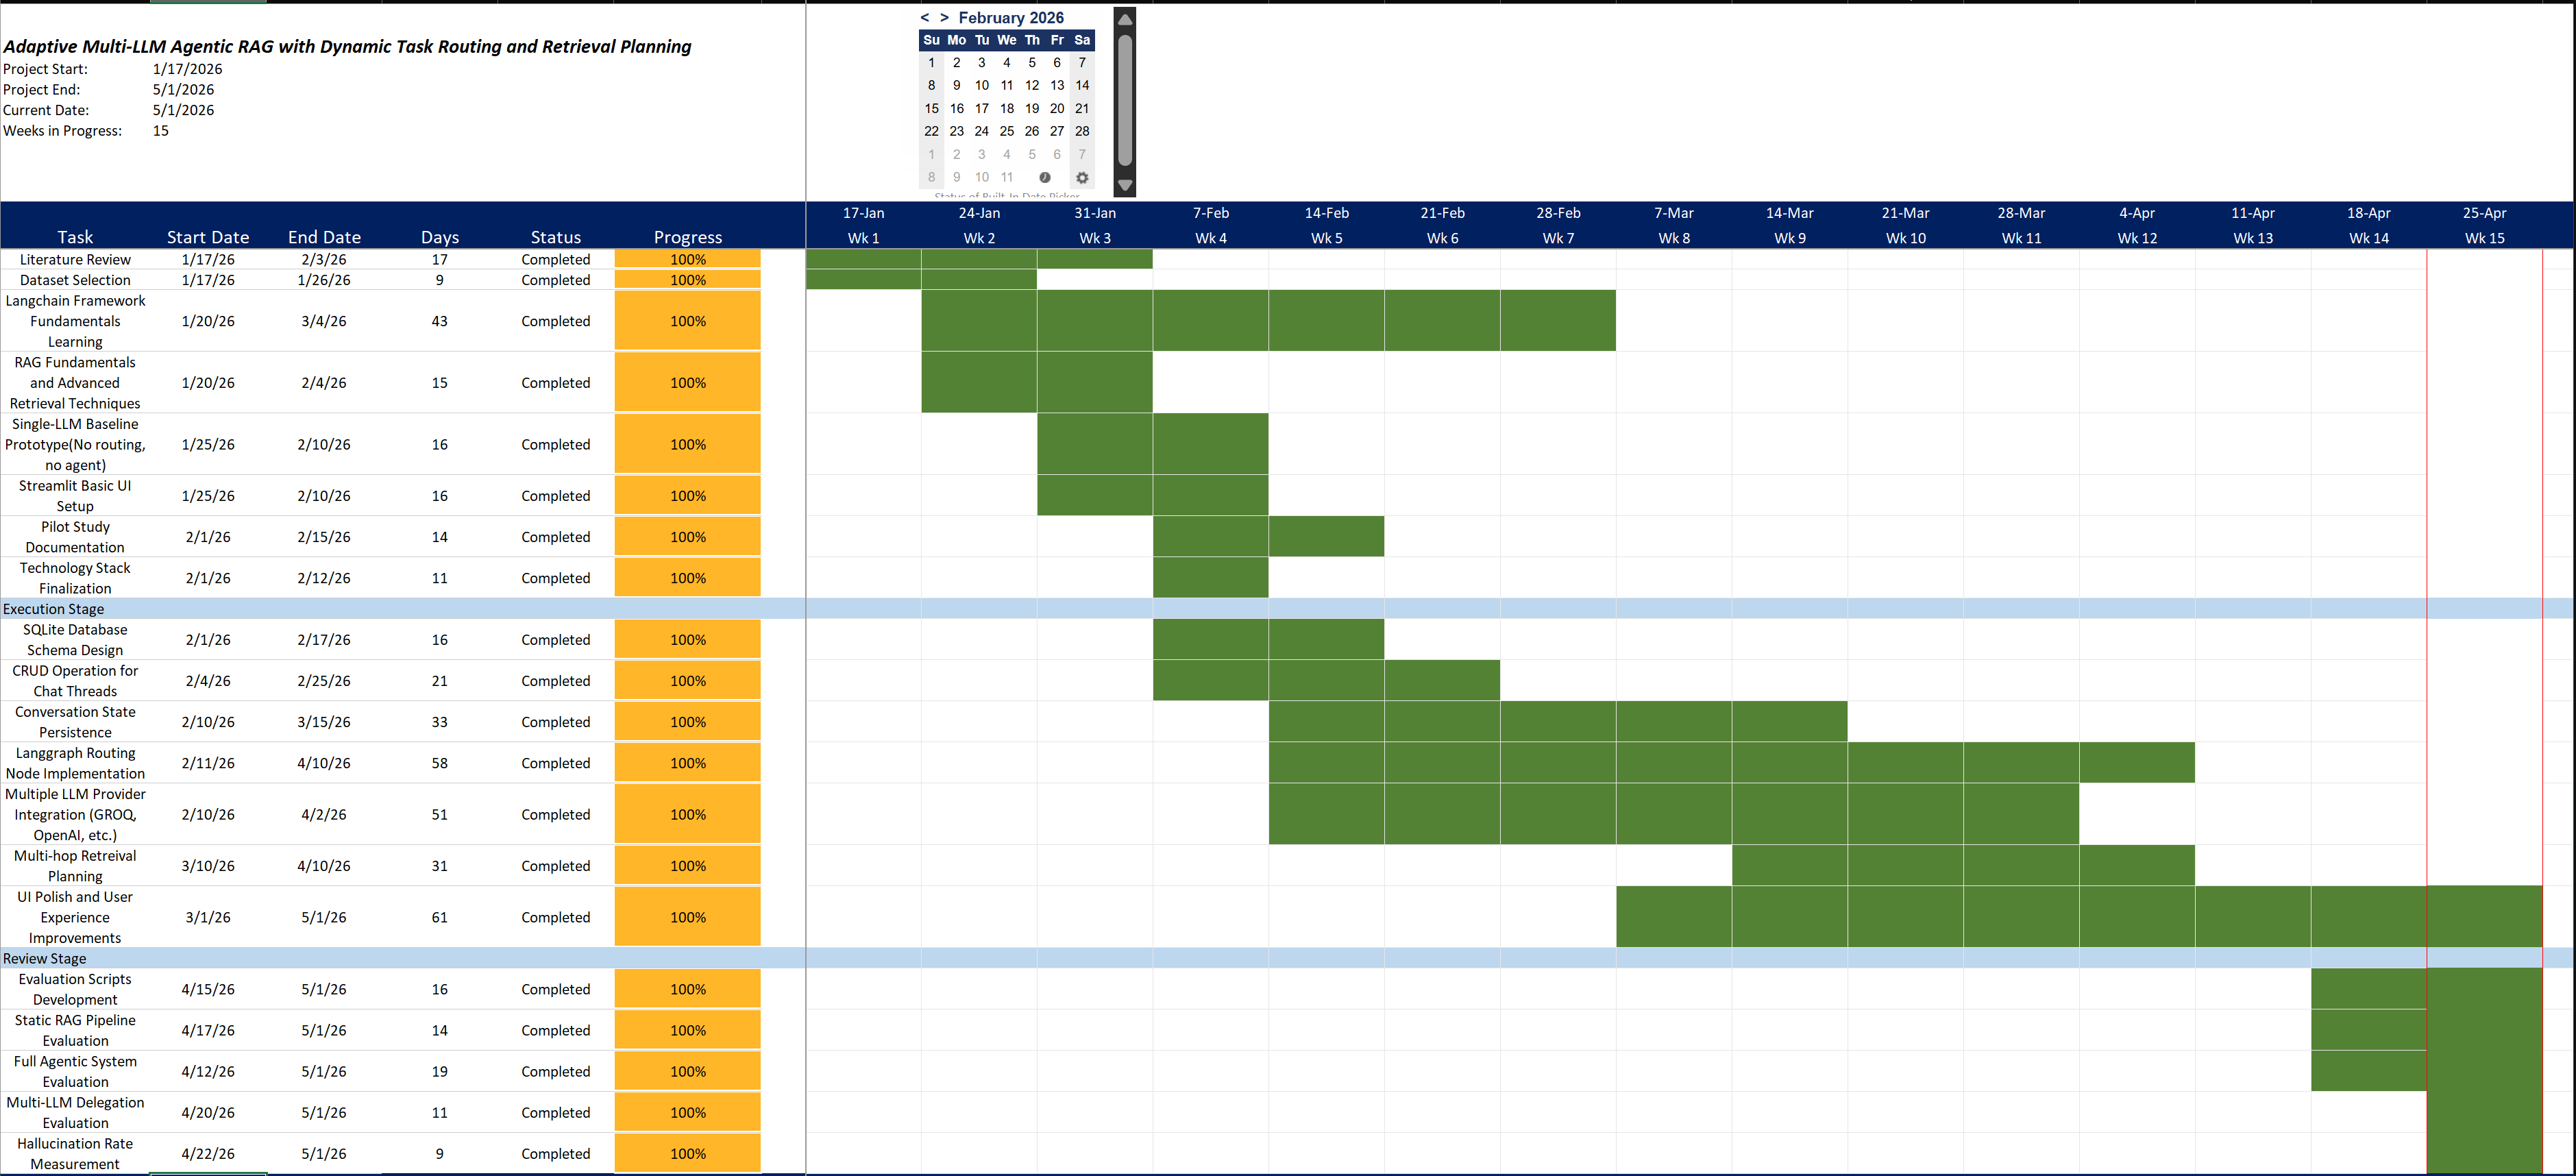
\includegraphics[width=\textwidth]{../assets/gnatt_chart.png}
    \caption{Project Gantt Chart illustrating the full project timeline from January 17, 2026 to May 2, 2026.}
    \label{fig:gantt_chart}
\end{figure}

\FloatBarrier

\newpage

% =================================================

\section{Conclusion}
\label{sec:conclusion}

This dissertation has presented the design, implementation, and evaluation of an Adaptive Multi-LLM Agentic RAG system that addresses the inefficiencies of monolithic conversational AI architectures. The system integrates ten heterogeneous language models within a LangGraph-based orchestration framework, dynamically routing queries to specialist models based on inferred task intent and complexity.

Key contributions include an intent-aware routing architecture distinguishing between direct inference, RAG, and agentic execution paths; a specialist model selection mechanism matched to task category and complexity; a MySQL-backed persistent checkpointing system for multi-user conversation management; a ChromaDB-based adaptive RAG pipeline; and a companion Android application via a FastAPI REST interface.

Experimental evaluation on HotpotQA and MuSiQue benchmarks demonstrates that the adaptive multi-LLM configuration improves accuracy for task-typed queries while maintaining competitive latency through lightweight model selection for low-complexity requests. The system provides a practical, deployable foundation for future research into cost-aware, quality-optimising conversational AI, with promising directions including learned routing classifiers, graph-based RAG, and extended benchmark evaluation.

\newpage

% =================================================


\section*{References}
\addcontentsline{toc}{section}{References}

\setlength{\parindent}{0pt}
\setlength{\parskip}{0.8em}

\justifying
\sloppy

% -------------------------------------------------
% References cited in the Introduction
% -------------------------------------------------

BROWN, T., MANN, B., RYDER, N., SUBBIAH, M., KAPLAN, J.D., DHARIWAL, P., NEELAKANTAN, A., SHYAM, P., SASTRY, G., ASKELL, A. et al., 2020. Language models are few-shot learners. \textit{Advances in Neural Information Processing Systems}, 33, pp. 1877--1901. Available from: \url{https://arxiv.org/abs/2005.14165}

WEI, J., WANG, X., SCHUURMANS, D., BOSMA, M., ICHTER, B., XIA, F., CHI, E., LE, Q. and ZHOU, D., 2022. Chain-of-thought prompting elicits reasoning in large language models. \textit{Advances in Neural Information Processing Systems}, 35, pp. 24824--24837. Available from: \url{https://arxiv.org/abs/2201.11903}

TOUVRON, H., LAVRIL, T., IZACARD, G., MARTINET, X., LACHAUX, M.A., LACROIX, T., ROZIÈRE, B., GOYAL, N., HAMBRO, E., AZHAR, F. et al., 2023. LLaMA: Open and efficient foundation language models. \textit{arXiv preprint arXiv:2302.13971}. Available from: \url{https://arxiv.org/abs/2302.13971}

JIANG, A.Q., SABLAYROLLES, A., MENSCH, A., BAMFORD, C., CHAPLOT, D.S., DE LAS CASAS, D., BRESSAND, F., LENGYEL, G., LAMPLE, G., SAULNIER, L. et al., 2023. Mistral 7B. \textit{arXiv preprint arXiv:2310.06825}. Available from: \url{https://arxiv.org/abs/2310.06825}

TEAM, G., ANIL, R., BORGEAUD, S., ALAYRAC, J.B., YU, J., SORICUT, R., SCHALKWYK, J., DAI, A.M., HAUTH, A., MILLICAN, K. et al., 2024. Gemini: A family of highly capable multimodal models. \textit{arXiv preprint arXiv:2312.11805}. Available from: \url{https://arxiv.org/abs/2312.11805}

SINGH, A., EHTESHAM, A., KUMAR, S. and TALAEI KHOEI, T., 2025. Agentic Retrieval-Augmented Generation: A survey on Agentic RAG. \textit{arXiv preprint arXiv:2501.09136}. Available from: \url{https://arxiv.org/abs/2501.09136}

LEWIS, P., PEREZ, E., PIKTUS, A., PETRONI, F., KARPUKHIN, V., GOYAL, N., KÜTTLER, H., LEWIS, M., YIH, W., ROCKTÄSCHEL, T. et al., 2020. Retrieval-augmented generation for knowledge-intensive NLP tasks. \textit{Advances in Neural Information Processing Systems}, 33, pp. 9459--9474. Available from: \url{https://arxiv.org/abs/2005.11401}

SHI, F., CHEN, X., MISRA, K., SCALES, N., DOHAN, D., CHI, E.H., SCHARLI, N. and ZHOU, D., 2023. Large language models can be easily distracted by irrelevant context. \textit{Proceedings of the 40th International Conference on Machine Learning}, pp. 31210--31227. Available from: \url{https://arxiv.org/abs/2302.00093}

ASAI, A., WU, Z., WANG, Y., SRINIVASAN, V., JIN, H., CHOI, Y. and HAJISHIRZI, H., 2023. Self-RAG: Learning to retrieve, generate, and critique through self-reflection. \textit{arXiv preprint arXiv:2310.11511}. Available from: \url{https://arxiv.org/abs/2310.11511}

YAO, S., ZHAO, J., YU, D., DU, N., SHAFRAN, I., NARASIMHAN, K. and CAO, Y., 2023. ReAct: Synergizing reasoning and acting in language models. \textit{Proceedings of the 11th International Conference on Learning Representations}. Available from: \url{https://arxiv.org/abs/2210.03629}

ZHAO, L., WANG, H., CHEN, Y., ZHANG, Y., CHEN, J. and HU, B., 2024. LangGraph: A framework for building stateful, multi-actor applications with LLMs. \textit{GitHub repository}. Available from: \url{https://github.com/langchain-ai/langgraph}

JEONG, S., BAEK, J., CHO, S., HWANG, S.J. and PARK, J.C., 2024. Adaptive-RAG: Learning to adapt retrieval-augmented large language models through question complexity. \textit{arXiv preprint arXiv:2403.14403}. Available from: \url{https://arxiv.org/abs/2403.14403}

% -------------------------------------------------
% References cited in the Literature Review only
% -------------------------------------------------

VASWANI, A., SHAZEER, N., PARMAR, N., USZKOREIT, J., JONES, L., GOMEZ, A.N., KAISER, Ł. and POLOSUKHIN, I., 2017. Attention is all you need. \textit{Advances in Neural Information Processing Systems}, 30. Available from: \url{https://arxiv.org/abs/1706.03762}

OUYANG, L., WU, J., JIANG, X., ALMEIDA, D., WAINWRIGHT, C., MISHKIN, P., ZHANG, C., AGARWAL, S., SLAMA, K., RAY, A. et al., 2022. Training language models to follow instructions with human feedback. \textit{Advances in Neural Information Processing Systems}, 35, pp. 27730--27744. Available from: \url{https://arxiv.org/abs/2203.02155}

ABDIN, M., ANEJA, J., AWADALLA, H., AWADALLAH, A., AWAN, A.A., BACH, N., BAHREE, A., BAKHTIARI, A., BAO, J., BEHL, H. et al., 2024. Phi-3 technical report: A highly capable language model locally on your phone. \textit{arXiv preprint arXiv:2404.14219}. Available from: \url{https://arxiv.org/abs/2404.14219}

KARPUKHIN, V., OGUZ, B., MIN, S., LEWIS, P., WU, L., EDUNOV, S., CHEN, D. and YIH, W., 2020. Dense passage retrieval for open-domain question answering. \textit{Proceedings of the 2020 Conference on EMNLP}, pp. 6769--6781. Available from: \url{https://arxiv.org/abs/2004.04906}

IZACARD, G. and GRAVE, E., 2021. Leveraging passage retrieval with generative models for open domain question answering. \textit{Proceedings of the 16th Conference of the European Chapter of the ACL}, pp. 874--880. Available from: \url{https://arxiv.org/abs/2007.01282}

ZHANG, N., ZHANG, C., TAN, Z., YANG, X., DENG, W. and WANG, W., 2025. Credible plan-driven RAG method for multi-hop question answering. \textit{arXiv preprint arXiv:2504.16787}. Available from: \url{https://arxiv.org/abs/2504.16787}

PARANJAPE, B., LUNDBERG, S., SINGH, S., HAJISHIRZI, H., ZETTLEMOYER, L. and RIBEIRO, M.T., 2023. ART: Automatic multi-step reasoning and tool-use for large language models. \textit{arXiv preprint arXiv:2303.09014}. Available from: \url{https://arxiv.org/abs/2303.09014}

ZOU, J., YANG, L., QI, Y., CHEN, S., AI, M., SHEN, K., HE, J. and WANG, M., 2025. AutoTool: Dynamic tool selection and integration for agentic reasoning. \textit{arXiv preprint arXiv:2508.xxxxx}. Available from: \url{https://arxiv.org/abs/2508.xxxxx}

CHEN, Y., ZHANG, E., YAN, L., WANG, S., HUANG, J., YIN, D. and MAO, J., 2025. MAO-ARAG: Multi-Agent Orchestration for Adaptive Retrieval-Augmented Generation. \textit{arXiv preprint arXiv:2508.01005}. Available from: \url{https://arxiv.org/abs/2508.01005}

NGUYEN, T., CHIN, P. and TAI, Y.-W., 2025. MA-RAG: Multi-Agent Retrieval-Augmented Generation via Collaborative Chain-of-Thought Reasoning. \textit{arXiv preprint arXiv:2505.20096}. Available from: \url{https://arxiv.org/abs/2505.20096}

XIONG, G., JIN, Q., WANG, X., FANG, Y., LIU, H., YANG, Y., CHEN, F., SONG, Z., WANG, D., ZHANG, M., LU, Z. and ZHANG, A., 2025. RAG-Gym: Systematic Optimization of Language Agents for Retrieval-Augmented Generation. \textit{arXiv preprint arXiv:2502.13957}. Available from: \url{https://arxiv.org/abs/2502.13957}

WANG, J., WANG, X., JAVAHERIPI, M., CORIA, R., SHAN, Y. and HAN, J., 2024. Mixture-of-Agents enhances large language model capabilities. \textit{arXiv preprint arXiv:2406.04692}. Available from: \url{https://arxiv.org/abs/2406.04692}

DING, D., MALLINAR, N., HAUGEN, M., SAHOO, O. and MAJI, S., 2024. Hybrid LLM: Cost-efficient and quality-aware query routing. \textit{arXiv preprint arXiv:2404.14618}. Available from: \url{https://arxiv.org/abs/2404.14618}

CHASE, H., 2022. LangChain. \textit{GitHub repository}. Available from: \url{https://github.com/langchain-ai/langchain}

YANG, Z., QI, P., ZHANG, S., BENGIO, Y., COHEN, W.W., SALAKHUTDINOV, R. and MANNING, C.D., 2018. HotpotQA: A dataset for diverse, explainable multi-hop question answering. \textit{Proceedings of the 2018 Conference on EMNLP}, pp. 2369--2380. Available from: \url{https://arxiv.org/abs/1809.09600}

TRIVEDI, H., BALASUBRAMANIAN, N., KHOT, T. and SABHARWAL, A., 2022. MuSiQue: Multihop questions via single-hop question composition. \textit{Transactions of the Association for Computational Linguistics}, 10, pp. 539--554. Available from: \url{https://arxiv.org/abs/2108.00573}

JI, Z., LEE, N., FRIESKE, R., YU, T., SU, D., XU, Y., ISHII, E., BANG, Y.J., MADOTTO, A. and FUNG, P., 2023. Survey of hallucination in natural language generation. \textit{ACM Computing Surveys}, 55(12), pp. 1--38.

HUANG, L., YU, W., MA, W., ZHONG, W., FENG, Z., WANG, H., CHEN, Q., PENG, W., FENG, X., QIN, B. and LIU, T., 2023. A survey on hallucination in large language models: Principles, taxonomy, challenges, and open questions. \textit{arXiv preprint arXiv:2311.05232}. Available from: \url{https://arxiv.org/abs/2311.05232}

HOWARD, A., SANDLER, M., CHU, G., CHEN, L.-C., CHEN, B., TAN, M., WANG, W., ZHU, Y., PANG, R., VASUDEVAN, V. et al., 2019. Searching for MobileNetV3. \textit{Proceedings of the IEEE/CVF International Conference on Computer Vision}, pp. 1314--1324.

% =================================================
% Appendix
% =================================================
\newpage
\appendix

\section{Dataset Access and Supplementary Resources}
\label{app:datasets}

\subsection{Benchmark Datasets}

The following publicly available datasets were used for system evaluation in this dissertation.

HotpotQA is available from: \url{https://hotpotqa.github.io/}. The dataset contains 113,000 Wikipedia-based multi-hop questions with supporting fact annotations, available in full-wiki and distractor settings.

MuSiQue is available from: \url{https://github.com/StonyBrookNLP/musique}. The dataset contains 2,417 compositional multi-hop questions with 2--4 reasoning hops, with both answerable and unanswerable variants.

\subsection{GitHub Repository}

The complete source code for this dissertation project, including the LangGraph chatbot implementation, FastAPI backend, evaluation scripts, and configuration files, is available at:

\textbf{GitHub Repository:} \texttt{[https://github.com/parthaAtSolent/COM726---Dissertation]}

The repository includes a comprehensive \texttt{README.md} with installation instructions, environment configuration guidance, and instructions for reproducing the benchmark evaluation results.

\subsection{Ethics Application}
\label{app:ethics}

The approved ethics application for this dissertation is provided below.

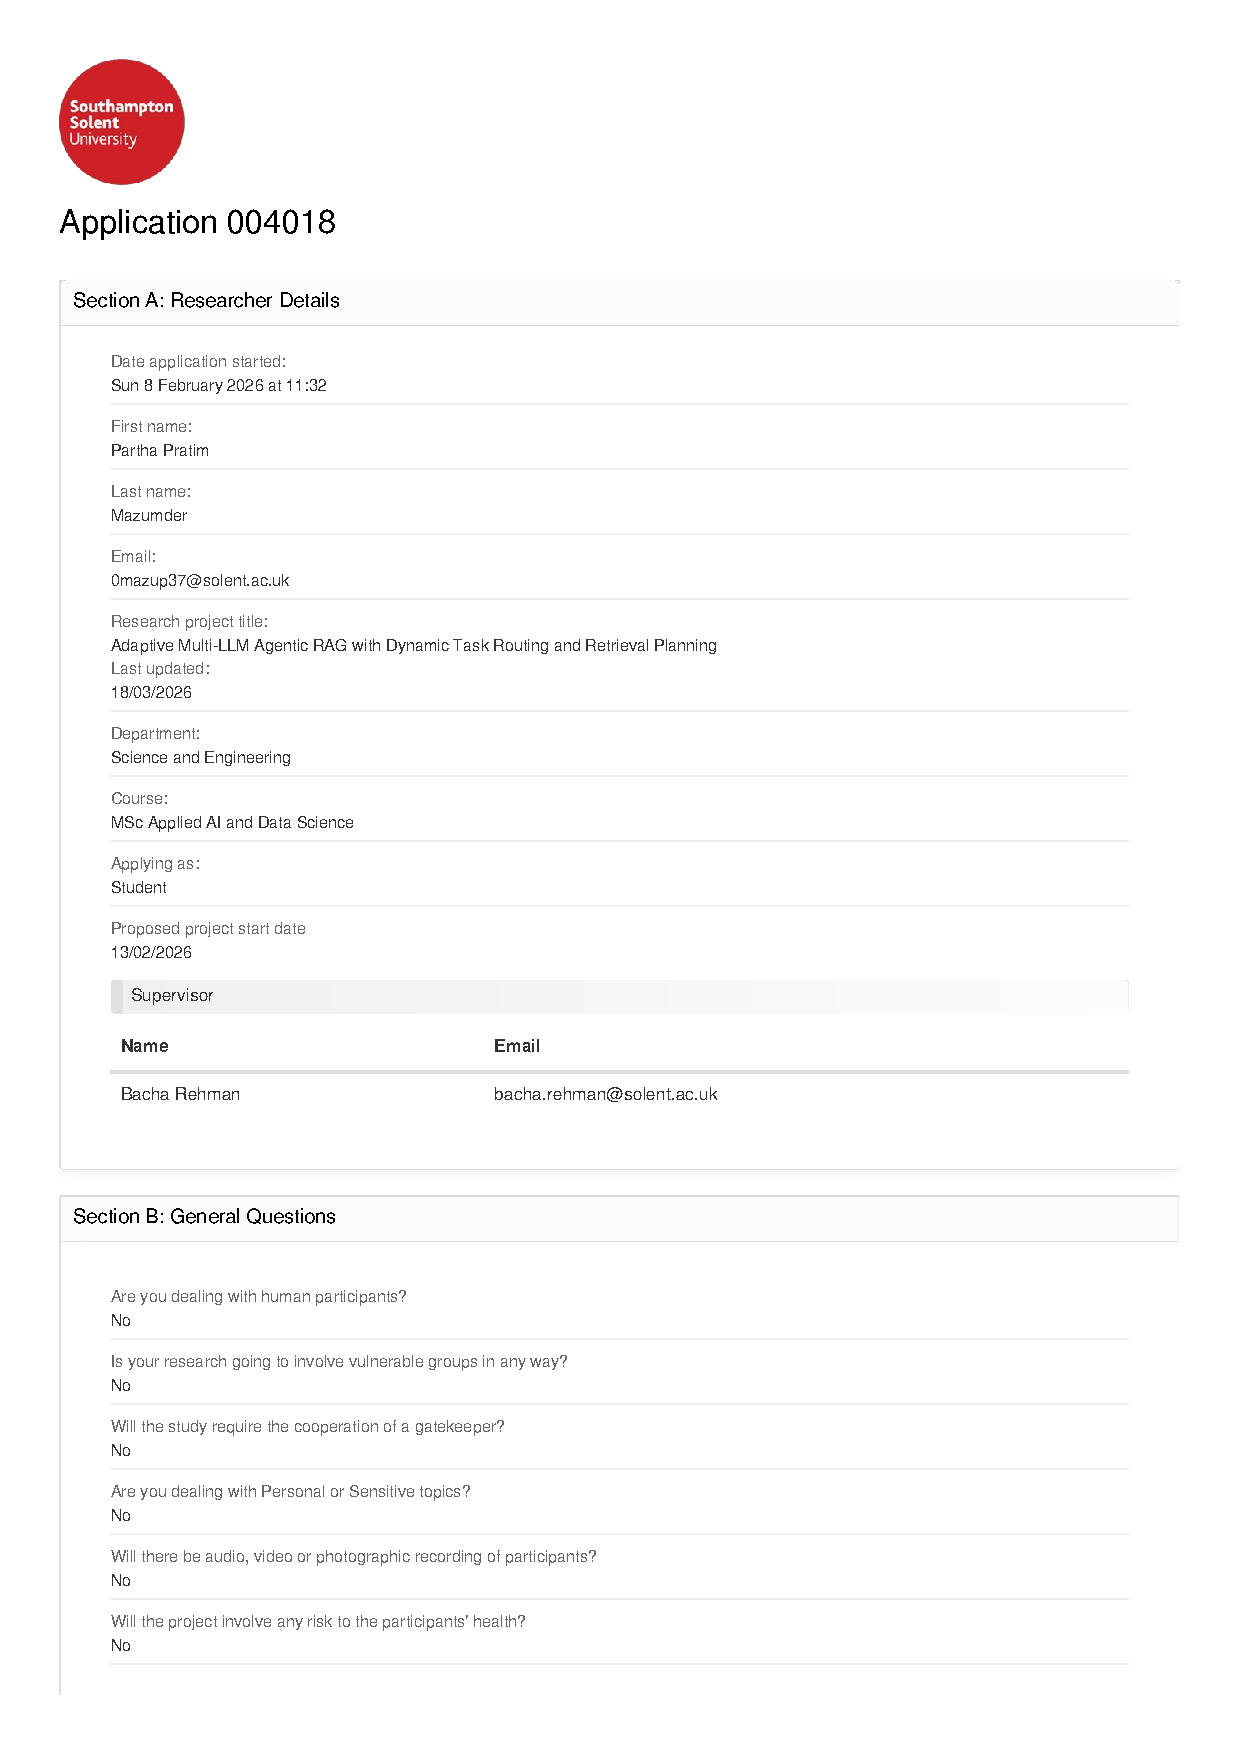
\includepdf[pages=-]{Ethics_Application.pdf}
\end{document}